\section{渐近评价}\label{sec:10}
\chapterdoi{10}
\sourcepageanchor{408}
\begin{quote}
我知道，亲爱的华生，你和我一样，喜爱一切离奇的、超出日常生活惯例与单调常规的事物.
\begin{flushright}夏洛克·福尔摩斯\\《红发会》\end{flushright}
\end{quote}

迄今为止，我们考虑的所有准则都是有限样本准则. 相比之下，也可以考虑渐近性质（asymptotic properties），即描述样本量趋于无穷时某一程序行为的性质. 本节考察其中一些性质，分别讨论点估计、假设检验与区间估计. 我们将特别强调最大似然程序的渐近性质.

渐近评价的力量在于，令样本量趋于无穷会使计算简化. 有限样本情形下无法完成的评价，变成了常规计算. 这种简化也让我们得以考察其他一些技术（如自助法和$M$估计），它们通常只能进行渐近评价.

让样本量无限增大（有时称为“渐近乌托邦”，asymptopia），不应被嘲笑为仅仅是一种异想天开的练习. 相反，渐近理论揭示一个程序最根本的性质，为我们提供极有力且普遍的评价工具.
\subsection{点估计}\label{sec:10.1}
\subsubsection{相合性}\label{sec:10.1.1}

相合性（consistency）似乎是一项十分基本的性质，它要求样本量趋于无穷时，估计量收敛到“正确”值. 这项性质如此基本，以至于不相合估计量的价值应受到质疑（或至少应受到认真研究）.

相合性（以及所有渐近性质）涉及的是估计量序列，而非单个估计量，尽管人们常说“相合估计量”. 若按照分布$f(x\mid\theta)$观测$X_1,X_2,\ldots$，只须对每个样本量$n$执行同一种估计程序，就能构造估计量序列$W_n=W_n(X_1,\ldots,X_n)$. 例如，$\bar X_1=X_1$，$\bar X_2=(X_1+X_2)/2$，$\bar X_3=(X_1+X_2+X_3)/3$，等等. 现在可以定义相合序列.

\begin{definition}\label{def:10.1.1}\index{SI0770@相合}
若对每个$\varepsilon>0$及每个$\theta\in\Theta$，估计量序列$W_n=W_n(X_1,\ldots,X_n)$满足
\begin{equation}\label{eq:10.1.1}
\lim_{n\to\infty}P_\theta(|W_n-\theta|<\varepsilon)=1,
\end{equation}
则称它为参数$\theta$的相合估计量序列.
\end{definition}

非正式地说，\eqref{eq:10.1.1}意味着，当样本量趋于无穷（样本信息越来越好）时，估计量会以很高的概率任意接近参数，这显然是理想的性质. 或者反过来说，相合估计量序列偏离真实参数的概率很小.
\sourcepageanchor{409}
与\eqref{eq:10.1.1}等价的表述如下：对每个$\varepsilon>0$及每个$\theta\in\Theta$，相合序列$W_n$满足
\begin{equation}\label{eq:10.1.2}
\lim_{n\to\infty}P_\theta(|W_n-\theta|\geq\varepsilon)=0.
\end{equation}
应将\autoref{def:10.1.1}与定义依概率收敛的\autoref{def:5.5.1}比较. \autoref{def:10.1.1}说，相合估计量序列依概率收敛到它所估计的参数$\theta$. \autoref{def:5.5.1}处理的是一个概率结构下的一列随机变量，而\autoref{def:10.1.1}处理的是由$\theta$标记的一整族概率结构. 对不同的$\theta$值，与序列$W_n$相关的概率结构不同. 定义要求，对每个$\theta$值，该概率结构均使序列依概率收敛到真实的$\theta$. 这就是概率定义与统计定义之间通常的区别：概率定义处理一个概率结构，统计定义处理一整族.

\begin{example}[$\bar X$的相合性]\label{ex:10.1.2}\index{SI0772@正态}
设$X_1,X_2,\ldots$独立同分布于$\mathrm n(\theta,1)$，考虑序列
$$\bar X_n=\frac1n\sum_{i=1}^nX_i.$$
回顾$\bar X_n\sim\mathrm n(\theta,1/n)$，所以
\begin{align*}
P_\theta(|\bar X_n-\theta|<\varepsilon)
&=\int_{\theta-\varepsilon}^{\theta+\varepsilon}\left(\frac n{2\pi}\right)^{1/2}e^{-(n/2)(\bar x_n-\theta)^2}\,d\bar x_n &&\text{（定义）}\\
&=\int_{-\varepsilon}^{\varepsilon}\left(\frac n{2\pi}\right)^{1/2}e^{-(n/2)y^2}\,dy &&\text{（代入$y=\bar x_n-\theta$）}\\
&=\int_{-\varepsilon\sqrt n}^{\varepsilon\sqrt n}\left(\frac1{2\pi}\right)^{1/2}e^{-t^2/2}\,dt &&\text{（代入$t=y\sqrt n$）}\\
&=P(-\varepsilon\sqrt n<Z<\varepsilon\sqrt n) &&(Z\sim\mathrm n(0,1))\\
&\longrightarrow1\quad\text{当$n\to\infty$}.
\end{align*}
因此，$\bar X_n$是$\theta$的相合估计量序列.
\end{example}

一般而言，验证相合性并不需要上面那样的详细计算.\index{SI0565@切比雪夫}\semanticindexanchor{565:409} 回顾切比雪夫不等式，对估计量$W_n$有
$$P_\theta(|W_n-\theta|\geq\varepsilon)\leq\frac{E_\theta[(W_n-\theta)^2]}{\varepsilon^2},$$
因此，若对每个$\theta\in\Theta$，
$$\lim_{n\to\infty}E_\theta[(W_n-\theta)^2]=0,$$
则该估计量序列相合. 此外，由\eqref{eq:7.3.1}，
\begin{equation}\label{eq:10.1.3}
E_\theta[(W_n-\theta)^2]=\operatorname{Var}_\theta W_n+[\operatorname{Bias}_\theta W_n]^2.
\end{equation}
综合这些事实，可以陈述如下定理.

\begin{theorem}\label{thm:10.1.3}
若$W_n$是参数$\theta$的估计量序列，且对每个$\theta\in\Theta$满足
\begin{enumerate}[label=\roman*.]
\item $\lim_{n\to\infty}\operatorname{Var}_\theta W_n=0$，
\item $\lim_{n\to\infty}\operatorname{Bias}_\theta W_n=0$，
\end{enumerate}
则$W_n$是$\theta$的相合估计量序列.
\end{theorem}

\sourcepageanchor{410}
\begin{example}[续\autoref{ex:10.1.2}]\label{ex:10.1.4}
因为
$$E_\theta\bar X_n=\theta\quad\text{且}\quad\operatorname{Var}_\theta\bar X_n=\frac1n,$$
所以满足\autoref{thm:10.1.3}的条件，序列$\bar X_n$相合. 此外，由\autoref{thm:5.2.6}，若从任意均值为$\theta$的总体中独立同分布抽样，只要总体方差有限，$\bar X_n$就相合地估计$\theta$.
\end{example}

本节开头说过，不相合估计量序列的价值应受到质疑. 这一说法的部分依据在于，相合序列如此之多，下面的定理说明了这一点. 证明留作\autoref{exercise:10.2}.

\begin{theorem}\label{thm:10.1.5}
设$W_n$是参数$\theta$的相合估计量序列，$a_1,a_2,\ldots$与$b_1,b_2,\ldots$是满足以下条件的常数序列：
\begin{enumerate}[label=\roman*.]
\item $\lim_{n\to\infty}a_n=1$，且
\item $\lim_{n\to\infty}b_n=0$.
\end{enumerate}
则序列$U_n=a_nW_n+b_n$是$\theta$的相合估计量序列.
\end{theorem}

本节最后概述一个关于最大似然估计量相合性的更一般的结果. 它表明，MLE是其参数的相合估计量；这是我们首次看到，寻找估计量的方法本身能够保证一种最优性性质.

要使MLE相合，基础密度（似然函数）必须满足某些“正则条件”（regularity conditions）. 这里不展开，详见\hyperref[sec:10.6.2]{杂录10.6.2}.

\begin{theorem}[MLE的相合性]\label{thm:10.1.6}\index{SI0674@相合性}\index{SI0771@最大似然估计量}
设$X_1,\ldots,X_n$独立同分布于$f(x\mid\theta)$，$L(\theta\mid\boldsymbol x)=\prod_{i=1}^nf(x_i\mid\theta)$为似然函数，$\hat\theta$为$\theta$的MLE，$\tau(\theta)$为$\theta$的连续函数. 在\hyperref[sec:10.6.2]{杂录10.6.2}对$f(x\mid\theta)$、从而对$L(\theta\mid\boldsymbol x)$施加的正则条件下，对每个$\varepsilon>0$及每个$\theta\in\Theta$，
$$\lim_{n\to\infty}P_\theta(|\tau(\hat\theta)-\tau(\theta)|\geq\varepsilon)=0.$$
即$\tau(\hat\theta)$是$\tau(\theta)$的相合估计量.
\end{theorem}
\begin{proof}
证明先说明，对每个$\theta\in\Theta$，$\frac1n\log L(\hat\theta\mid\boldsymbol x)$几乎处处收敛到$E_\theta(\log f(X\mid\theta))$. 在$f(x\mid\theta)$满足某些条件时，这意味着$\hat\theta$依概率收敛到$\theta$，从而$\tau(\hat\theta)$依概率收敛到$\tau(\theta)$. 详见\hyperref[bib:source311]{Stuart、Ord和Arnold（1999}，第18章）.
\end{proof}

\subsubsection{效率}\label{sec:10.1.2}\index{SI0394@效率（另见点估计）}\index{SI0779@效率}
相合性关心估计量的渐近准确性：它是否收敛到所估计的参数.\index{SI0071@渐近方差（另见方差）}\semanticindexanchor{71:410}\index{SI1063@渐近}\semanticindexanchor{1063:410} 本节考察相关的效率（efficiency）性质，它关心估计量的渐近方差.

计算渐近方差时，人们或许很容易采用如下做法. 给定基于样本量$n$的估计量$T_n$，先计算有限样本方差$\operatorname{Var}T_n$，再求$\lim_{n\to\infty}k_n\operatorname{Var}T_n$，其中$k_n$是某个规范化常数. （注意，在许多情形中，$n\to\infty$时$\operatorname{Var}T_n\to0$，所以需要因子$k_n$使它趋于一个极限.）

\begin{definition}\label{def:10.1.7}\index{SI1065@极限}
对估计量$T_n$，若$\lim_{n\to\infty}k_n\operatorname{Var}T_n=\tau^2<\infty$，其中$\{k_n\}$是常数序列，则称$\tau^2$为极限方差（limiting variance），或方差的极限（limit of the variances）.
\end{definition}

\begin{example}[极限方差]\label{ex:10.1.8}
对于$n$个独立同分布正态观测的均值$\bar X_n$，其中$EX=\mu$、$\operatorname{Var}X=\sigma^2$，若取$T_n=\bar X_n$，则$\lim\sqrt n\operatorname{Var}\bar X_n=\sigma^2$是$T_n$的极限方差.\footnote{译注：原文系数为$\sqrt n$；由$\operatorname{Var}\bar X_n=\sigma^2/n$可知，欲得到$\sigma^2$，此处应为$n$，而非$\sqrt n$. 原式保留.}

\sourcepageanchor{411}
但若改为用$1/\bar X_n$估计$1/\mu$，例如，就会出现麻烦. 此时取$T_n=1/\bar X_n$，会发现方差$\operatorname{Var}(T_n)=\infty$，因此方差的极限为无穷. 不过，回顾\autoref{ex:5.5.23}，其中说$1/\bar X_n$的“近似”均值和方差为
$$E\left(\frac1{\bar X_n}\right)\approx\frac1\mu,\qquad
\operatorname{Var}\left(\frac1{\bar X_n}\right)\approx\left(\frac1\mu\right)^4\operatorname{Var}\bar X_n,$$
于是，按第二种计算，方差为$\operatorname{Var}(T_n)\approx\sigma^2/(n\mu^4)<\infty$.
\end{example}

这个例子指出了把方差的极限作为大样本度量的问题. 当然，$1/\bar X$的精确有限样本方差为$\infty$. 然而，若$\mu\ne0$，$1/\bar X$变得非常大的区域，其概率趋于0. 所以\autoref{ex:10.1.8}中的第二种近似更符合实际（也更有用）. 我们采用的正是这第二种计算大样本方差的方法.

\begin{definition}\label{def:10.1.9}
对估计量$T_n$，假设$k_n(T_n-\mu)\to\mathrm n(0,\sigma^2)$. 参数$\sigma^2$称为$T_n$的渐近方差（asymptotic variance），或极限分布的方差（variance of the limit distribution）.
\end{definition}

计算样本均值及其他平均量的方差时，极限方差与渐近方差通常具有相同的值. 但在较复杂的情形中，极限方差有时会失效. 另一个有趣的事实是，渐近方差总是小于极限方差（\hyperref[bib:source200]{Lehmann和Casella，第6.1节}）. 下面给出说明.

\begin{example}[大样本混合方差]\label{ex:10.1.10}\index{SI1065@极限}
分层模型
$$\begin{aligned}
Y_n\mid W_n=w_n&\sim\mathrm n\bigl(0,w_n+(1-w_n)\sigma_n^2\bigr),\\
W_n&\sim\operatorname{Bernoulli}(p_n)
\end{aligned}$$
能够使渐近方差与极限方差出现很大差异. （有时也把它描述为混合模型，即以概率$p_n$观测到$Y_n\sim\mathrm n(0,1)$，以概率$1-p_n$观测到$Y_n\sim\mathrm n(0,\sigma_n^2)$.）

首先，由\autoref{thm:4.4.7}，
$$\operatorname{Var}(Y_n)=p_n+(1-p_n)\sigma_n^2.$$
由此可知，仅当$\lim_n(1-p_n)\sigma_n^2<\infty$时，$Y_n$的极限方差才有限.

另一方面，可利用
$$P(Y_n<a)=p_nP(Z<a)+(1-p_n)P(Z<a/\sigma_n)$$
直接计算$Y_n$的渐近分布. 现令$p_n\to1$且$\sigma_n\to\infty$，使$(1-p_n)\sigma_n^2\to\infty$. 则$P(Y_n<a)\to P(Z<a)$，即$Y_n\to\mathrm n(0,1)$，且
$$\begin{aligned}
\text{极限方差}&=\lim_n p_n+(1-p_n)\sigma_n^2=\infty,\\
\text{渐近方差}&=1.
\end{aligned}$$
更多细节见\autoref{exercise:10.6}.
\end{example}

仿照Cramér--Rao下界（\autoref{thm:7.3.9}）的思路，可以给出一个最优渐近方差.

\sourcepageanchor{412}
\begin{definition}\label{def:10.1.11}\index{SI0065@渐近效率}\index{SI0779@效率}
若估计量序列$W_n$满足$\sqrt n[W_n-\tau(\theta)]$依分布收敛到$\mathrm n[0,v(\theta)]$，且
$$v(\theta)=\frac{[\tau'(\theta)]^2}{E_\theta\left(\left(\frac\partial{\partial\theta}\log f(X\mid\theta)\right)^2\right)},$$
则称它对于参数$\tau(\theta)$渐近有效（asymptotically efficient）. 即$W_n$的渐近方差达到Cramér--Rao下界.
\end{definition}

回顾\autoref{thm:10.1.6}，它表明在一般条件下MLE相合. 在略强一些的正则条件下，关于渐近有效性也有同类定理成立，因此一般可以认为MLE既相合又渐近有效. 正则条件的细节仍见\hyperref[sec:10.6.2]{杂录10.6.2}.

\begin{theorem}[MLE的渐近有效性]\label{thm:10.1.12}\index{SI0668@渐近效率}\index{SI0796@渐近效率}
设$X_1,\ldots,X_n$独立同分布于$f(x\mid\theta)$，$\hat\theta$为$\theta$的MLE，$\tau(\theta)$为$\theta$的连续函数. 在\hyperref[sec:10.6.2]{杂录10.6.2}对$f(x\mid\theta)$、从而对$L(\theta\mid\boldsymbol x)$施加的正则条件下，
$$\sqrt n[\tau(\hat\theta)-\tau(\theta)]\longrightarrow\mathrm n[0,v(\theta)],$$
其中$v(\theta)$为Cramér--Rao下界. 即$\tau(\hat\theta)$是$\tau(\theta)$的相合且渐近有效的估计量.
\end{theorem}
\begin{proof}
这个定理的证明有趣之处在于使用泰勒级数，并利用MLE被定义为似然函数的零点这一事实.\footnote{译注：原文称“似然函数的零点”；按接下来的计算，应为对数似然函数的一阶导数的零点，即似然方程的根. 原文保留.} 我们概述$\hat\theta$渐近有效的证明；推广到$\tau(\hat\theta)$留作\autoref{exercise:10.7}.

回顾$l(\theta\mid\boldsymbol x)=\sum\log f(x_i\mid\theta)$为对数似然函数，将关于$\theta$的导数记为$l',l'',\ldots$. 现在在真值$\theta_0$处展开对数似然函数的一阶导数：
\begin{equation}\label{eq:10.1.4}
l'(\theta\mid\boldsymbol x)=l'(\theta_0\mid\boldsymbol x)+(\theta-\theta_0)l''(\theta_0\mid\boldsymbol x)+\cdots,
\end{equation}
我们将忽略高阶项（正则条件保证这种做法成立）.

现用MLE $\hat\theta$代替$\theta$，注意到\eqref{eq:10.1.4}左侧为零. 整理并乘以$\sqrt n$，得到
\begin{equation}\label{eq:10.1.5}
\sqrt n(\hat\theta-\theta_0)=\sqrt n\frac{-l'(\theta_0\mid\boldsymbol x)}{l''(\theta_0\mid\boldsymbol x)}
=\frac{\frac1{\sqrt n}l'(\theta_0\mid\boldsymbol x)}{-\frac1n l''(\theta_0\mid\boldsymbol x)}.
\end{equation}
若令$I(\theta_0)=E[l'(\theta_0\mid\boldsymbol X)]^2=1/v(\theta)$表示信息量，应用中心极限定理与大数定律可知（细节见\autoref{exercise:10.8}）\footnote{译注：这里$l$已定义为全样本对数似然，故其得分平方的期望为$n$倍的单个观测信息量. 要与下式及$1/v(\theta_0)$一致，定义中应使用单个观测的对数密度导数，或将$E\{[l'(\theta_0\mid\boldsymbol X)]^2\}$除以$n$. 原文还将$v$的自变量写成$\theta$，此处照录.}
\begin{equation}\label{eq:10.1.6}
\begin{aligned}
\frac1{\sqrt n}l'(\theta_0\mid\boldsymbol X)&\longrightarrow\mathrm n[0,I(\theta_0)]\quad\text{依分布},\\
\text{且}\qquad-\frac1n l''(\theta_0\mid\boldsymbol X)&\longrightarrow I(\theta_0)\quad\text{依概率}.
\end{aligned}
\end{equation}
因此，若令$W\sim\mathrm n[0,I(\theta_0)]$，则$\sqrt n(\hat\theta-\theta_0)$依分布收敛到$W/I(\theta_0)\sim\mathrm n[0,1/I(\theta_0)]$，定理得证.
\end{proof}

\begin{example}[渐近正态性与相合性]\label{ex:10.1.13}
上述定理表明，MLE通常有效且相合. 要指出的是，这种说法有些重复，因为效率仅在估计量渐近正态时才有定义，而正如下面所说明的，渐近正态性蕴含相合性. 假设
$$\sqrt n\frac{W_n-\mu}{\sigma}\longrightarrow Z\quad\text{依分布},$$
\sourcepageanchor{413}
其中$Z\sim\mathrm n(0,1)$. 应用Slutsky定理（\autoref{thm:5.5.17}），得到
$$W_n-\mu=\left(\frac\sigma{\sqrt n}\right)\left(\sqrt n\frac{W_n-\mu}{\sigma}\right)
\longrightarrow\lim_{n\to\infty}\left(\frac\sigma{\sqrt n}\right)Z=0,$$
因此$W_n-\mu$依分布收敛到0. 由\autoref{thm:5.5.13}，依分布收敛到一个点等价于依概率收敛，所以$W_n$是$\mu$的相合估计量.
\end{example}

\subsubsection{计算与比较}\label{sec:10.1.3}
前面各节导出的渐近公式，可以提供适合大样本使用的近似方差. 我们仍需关注正则条件（\hyperref[sec:10.6.2]{杂录10.6.2}），但这些条件相当一般，在通常情形下几乎总能满足. 不过，有一个条件值得特别强调；正如在\autoref{ex:7.3.13}中所见，违反它会造成复杂情况. 要使以下近似成立，pdf或pmf、从而似然函数的支撑集必须与参数无关.

假设MLE渐近有效，则\autoref{thm:10.1.6}中的渐近方差就是\autoref{thm:5.5.24}的Delta方法方差（去掉$1/n$项）.\footnote{译注：这里及本小节后文多次把渐近有效性归于\autoref{thm:10.1.6}；该定理只陈述相合性，渐近有效性在\autoref{thm:10.1.12}中陈述. 保留原书所引编号，后续同类引用不再逐一注释.} 因此，可以用Cramér--Rao下界近似MLE的真实方差. 假设$X_1,\ldots,X_n$独立同分布于$f(x\mid\theta)$，$\hat\theta$是$\theta$的MLE，而$I_n(\theta)=E_\theta\left(-\frac\partial{\partial\theta}\log L(\theta\mid\boldsymbol X)\right)^2$是样本信息量. 利用Delta方法与MLE的渐近有效性，$h(\hat\theta)$的方差可近似为
\begin{equation}\label{eq:10.1.7}\index{SI0582@信息量}
\begin{aligned}
\operatorname{Var}(h(\hat\theta)\mid\theta)
&\approx\frac{[h'(\theta)]^2}{I_n(\theta)}\\
&\approx\frac{[h'(\theta)]^2}{E_\theta\left(-\frac{\partial^2}{\partial\theta^2}\log L(\theta\mid\boldsymbol X)\right)}
&&\text{（使用\autoref{lem:7.3.11}的恒等式）}\\
&\approx\frac{[h'(\theta)]^2|_{\theta=\hat\theta}}{-\frac{\partial^2}{\partial\theta^2}\log L(\theta\mid\boldsymbol X)|_{\theta=\hat\theta}}
&&\text{（分母为观测信息量$\hat I_n(\hat\theta)$）}.
\end{aligned}
\end{equation}
此外，已有结果表明（\hyperref[bib:source110]{Efron和Hinkley，1978）}，使用观测信息量（observed information number）优于使用期望信息量（expected information number），后者正是Cramér--Rao下界中的信息量.

注意，方差估计分为两步，只是在\eqref{eq:10.1.7}中这一点不太明显. 为估计$\operatorname{Var}_\theta h(\hat\theta)$，先近似$\operatorname{Var}_\theta h(\hat\theta)$，再估计所得近似，通常用$\hat\theta$代入$\theta$. 所得估计可记为$\operatorname{Var}_{\hat\theta}h(\hat\theta)$或$\widehat{\operatorname{Var}}_\theta h(\hat\theta)$.

由\autoref{thm:10.1.6}，$-\frac1n\frac{\partial^2}{\partial\theta^2}\log L(\theta\mid\boldsymbol X)|_{\theta=\hat\theta}$是$I(\theta)$的相合估计量，故$\widehat{\operatorname{Var}}_\theta h(\hat\theta)$是$\operatorname{Var}_\theta h(\hat\theta)$的相合估计量.

\begin{example}[近似二项方差]\label{ex:10.1.14}\index{SI0670@近似方差}
在\autoref{ex:7.2.7}中看到，$\hat p=\sum X_i/n$是$p$的MLE，其中$X_1,\ldots,X_n$为来自Bernoulli$(p)$总体的随机样本. 直接计算也知道
$$\operatorname{Var}_p\hat p=\frac{p(1-p)}n,$$
而$\operatorname{Var}_p\hat p$的一个合理估计为
\begin{equation}\label{eq:10.1.8}
\widehat{\operatorname{Var}}_p\hat p=\frac{\hat p(1-\hat p)}n.
\end{equation}
\sourcepageanchor{414}
若应用\eqref{eq:10.1.7}的近似，取$h(p)=p$，则得到$\operatorname{Var}_p\hat p$的估计
$$\widehat{\operatorname{Var}}_p\hat p\approx\frac1{-\frac{\partial^2}{\partial p^2}\log L(p\mid\boldsymbol x)|_{p=\hat p}}.$$
回顾
$$\log L(p\mid\boldsymbol x)=n\hat p\log(p)+n(1-\hat p)\log(1-p),$$
因此\footnote{译注：下面二阶导数的第二项原文分子为$n(1-p)$；对上式求导应为$n(1-\hat p)$. 随后的$p=\hat p$代入式是相符的. 此处保留原式.}
$$\frac{\partial^2}{\partial p^2}\log L(p\mid\boldsymbol x)=-\frac{n\hat p}{p^2}-\frac{n(1-p)}{(1-p)^2}.$$
在$p=\hat p$处计算二阶导数，得到
$$\left.\frac{\partial^2}{\partial p^2}\log L(p\mid\boldsymbol x)\right|_{p=\hat p}
=-\frac{n\hat p}{\hat p^2}-\frac{n(1-\hat p)}{(1-\hat p)^2}=-\frac n{\hat p(1-\hat p)},$$
给出的方差近似与\eqref{eq:10.1.8}完全相同. 现在可以应用\autoref{thm:10.1.6}断言$\hat p$渐近有效，特别是
$$\sqrt n(\hat p-p)\longrightarrow\mathrm n[0,p(1-p)]$$
依分布成立. 若再用\autoref{thm:5.5.17}（Slutsky定理），则有
$$\sqrt n\frac{\hat p-p}{\sqrt{\hat p(1-\hat p)}}\longrightarrow\mathrm n[0,1].$$

估计$\hat p$的方差其实并不难，无须动用这些近似的全部工具. 不过，若转向稍复杂一些的函数，事情就可能棘手起来. 回顾\hyperref[ex:5.5.22]{习题5.5.22}\footnote{译注：原文称“习题5.5.22”，实际对应\autoref{ex:5.5.22}. 原称呼保留，链接指向对应例.}，其中用Delta方法近似$\hat p/(1-\hat p)$的方差，该量估计优势比$p/(1-p)$.\index{SI0728@优势}\semanticindexanchor{728:414} 现在可知，这个估计量实际上就是优势比的MLE，而且其方差可估计为
$$\begin{aligned}
\widehat{\operatorname{Var}}\left(\frac{\hat p}{1-\hat p}\right)
&\approx\frac{\left[\frac\partial{\partial p}\left(\frac p{1-p}\right)\right]^2\big|_{p=\hat p}}{-\frac{\partial^2}{\partial p^2}\log L(p\mid\boldsymbol x)|_{p=\hat p}}\\
&=\frac{\left[\frac{(1-p)+p}{(1-p)^2}\right]^2\big|_{p=\hat p}}{\frac n{p(1-p)}\big|_{p=\hat p}}
=\frac{\hat p}{n(1-\hat p)^3}.
\end{aligned}$$
此外，也知道该估计量渐近有效.
\end{example}

MLE方差近似在许多情形下表现很好，但并非万无一失. 特别是当函数$h(\hat\theta)$不单调时，必须谨慎. 这种情形下，导数$h'$会变号，可能导致低估方差的近似. 应认识到，这个近似基于Cramér--Rao下界，因此很可能本来就是低估；非单调函数会使问题更加严重.

\begin{example}[续\autoref{ex:10.1.14}]\label{ex:10.1.15}
现在假设要估计伯努利分布的方差$p(1-p)$. 该方差的MLE为$\hat p(1-\hat p)$，应用\eqref{eq:10.1.7}可估计这个估计量的方差：
$$\begin{aligned}
\widehat{\operatorname{Var}}\bigl(\hat p(1-\hat p)\bigr)
&\approx\frac{\left[\frac\partial{\partial p}(p(1-p))\right]^2\big|_{p=\hat p}}{-\frac{\partial^2}{\partial p^2}\log L(p\mid\boldsymbol x)|_{p=\hat p}}\\
&=\frac{(1-2p)^2|_{p=\hat p}}{\frac n{p(1-p)}\big|_{p=\hat p}}
=\frac{\hat p(1-\hat p)(1-2\hat p)^2}n,
\end{aligned}$$
当$\hat p=1/2$时它可能为零，显然低估了$\hat p(1-\hat p)$的方差. 函数$p(1-p)$不单调是造成这个问题的一个原因.

\sourcepageanchor{415}
利用\autoref{thm:10.1.6}，只要$p\ne1/2$，就能断言该估计量渐近有效. 若$p=1/2$，则需采用\autoref{thm:5.5.26}给出的二阶近似（见\autoref{exercise:10.10}）.
\end{example}

渐近有效性为我们希望达到的渐近方差提供一个基准\index{SI0780@有效}\semanticindexanchor{780:415}（不过见\hyperref[sec:10.6.1]{杂录10.6.1}）. 也可以通过渐近相对效率（asymptotic relative efficiency）的概念，利用渐近方差来比较估计量.

\begin{definition}\label{def:10.1.16}\index{SI0066@渐近相对效率}
若两个估计量$W_n$与$V_n$满足
$$\begin{aligned}
\sqrt n[W_n-\mu]&\longrightarrow\mathrm n[0,\sigma_W^2],\\
\sqrt n[V_n-\mu]&\longrightarrow\mathrm n[0,\sigma_V^2]
\end{aligned}$$
依分布成立，则$V_n$相对于$W_n$的渐近相对效率为
$$\operatorname{ARE}(V_n,W_n)=\frac{\sigma_W^2}{\sigma_V^2}.$$
\end{definition}

\begin{example}[泊松估计量的ARE]\label{ex:10.1.17}
假设$X_1,X_2,\ldots,X_n$独立同分布于Poisson$(\lambda)$，我们希望估计取零的概率. 例如，有时将给定时间段内进入银行的顾客人数建模为泊松随机变量，取零的概率就是一个时间段内无人进入银行的概率. 若$X\sim\operatorname{Poisson}(\lambda)$，则$P(X=0)=e^{-\lambda}$；一个自然（但有些朴素）的估计量来自定义$Y_i=I(X_i=0)$并采用
$$\hat\tau=\frac1n\sum_{i=1}^nY_i.$$
$Y_i$服从Bernoulli$(e^{-\lambda})$，所以
$$E(\hat\tau)=e^{-\lambda}\quad\text{且}\quad\operatorname{Var}(\hat\tau)=\frac{e^{-\lambda}(1-e^{-\lambda})}n.$$
另一种选择是$e^{-\lambda}$的MLE $e^{-\hat\lambda}$，其中$\hat\lambda=\sum_iX_i/n$是$\lambda$的MLE. 利用Delta方法近似，有
$$E(e^{-\hat\lambda})\approx e^{-\lambda}\quad\text{且}\quad\operatorname{Var}(e^{-\hat\lambda})\approx\frac{\lambda e^{-2\lambda}}n.$$
因为
$$\begin{aligned}
\sqrt n(\hat\tau-e^{-\lambda})&\longrightarrow\mathrm n[0,e^{-\lambda}(1-e^{-\lambda})],\\
\sqrt n(e^{-\hat\lambda}-e^{-\lambda})&\longrightarrow\mathrm n[0,\lambda e^{-2\lambda}]
\end{aligned}$$
依分布成立，所以$\hat\tau$相对于MLE $e^{-\hat\lambda}$的ARE为
$$\operatorname{ARE}(\hat\tau,e^{-\hat\lambda})=\frac{\lambda e^{-2\lambda}}{e^{-\lambda}(1-e^{-\lambda})}.$$
考察这个函数可知，它严格递减，在$\lambda=0$达到最大值1（这是$\hat\tau$所能达到的最佳情形），并随着$\lambda\to\infty$迅速下降、渐近趋于0，在$\lambda=4$时已低于10\%. （见\autoref{exercise:10.9}.）
\end{example}

\sourcepageanchor{416}
因为MLE通常渐近有效，另一个估计量无法指望在渐近方差上胜过它. 然而，其他估计量可能具有其他理想性质（计算方便、对基础假设稳健），使它们值得采用. 此时，MLE的效率就成为衡量使用替代估计量所付代价的重要标准.

我们再看最后一个例子，将计算方便与最优方差作比较. 下一节讨论稳健性问题.

\begin{example}[估计伽马均值]\label{ex:10.1.18}
尽管可能难以置信，估计伽马分布的均值并不是一件容易的事. 回顾伽马pdf $f(x\mid\alpha,\beta)$为
$$f(x\mid\alpha,\beta)=\frac1{\Gamma(\alpha)\beta^\alpha}x^{\alpha-1}e^{-x/\beta}.$$
其均值为$\alpha\beta$；要计算最大似然估计量，就必须处理伽马函数的导数（称为双伽马函数，digamma function），这从来不是令人愉快的事. 相比之下，矩方法给出容易计算的估计.

具体地，假设有来自上述伽马密度的随机样本$X_1,X_2,\ldots,X_n$，但重新参数化，使均值$\mu=\alpha\beta$显式出现. 此时
$$f(x\mid\mu,\beta)=\frac1{\Gamma(\mu/\beta)\beta^{\mu/\beta}}x^{\mu/\beta-1}e^{-x/\beta},$$
而$\mu$的矩估计量为$\bar X$，方差为$\beta\mu/n$.

为计算MLE，采用对数似然
$$l(\mu,\beta\mid\boldsymbol x)=\sum_{i=1}^n\log f(x_i\mid\mu,\beta).$$
为简化计算，假设$\beta$已知，故解$\frac d{d\mu}l(\mu,\beta\mid\boldsymbol x)=0$求MLE $\hat\mu$. 没有显式解，所以采用数值方法.

由\autoref{thm:10.1.6}，知道$\hat\mu$渐近有效. 关注的问题是，使用较容易计算的矩估计量会损失多少. 为作比较，计算渐近相对效率\footnote{译注：此处ARE公式与\autoref{def:10.1.16}及随后“大于1”的说法互有不一致. 按定义，$\operatorname{ARE}(\bar X,\hat\mu)$应为MLE渐近方差除以$\bar X$的渐近方差；若以单个观测信息量$I(\mu)$表示，应为$1/[I(\mu)\beta\mu]\leq1$. 原文公式使用全样本信息量作分子，图中又显示其倒数方向的效率损失. 保留原公式、文字与原图，待对照作者勘误核实.}
$$\operatorname{ARE}(\bar X,\hat\mu)=\frac{E\left(-\frac{d^2}{d\mu^2}l(\mu,\beta\mid\boldsymbol X)\right)}{\beta\mu},$$
并在\autoref{fig:10.1.1}中对若干$\beta$值画出它. 当然，知道ARE一定大于1，但从图中可以看到，对较大的$\beta$，进行更复杂的计算并使用MLE是值得的. （推广见\autoref{exercise:10.11}，计算细节见\autoref{ex:12.6.7}.）
\end{example}

\subsubsection{自助法标准误}\label{sec:10.1.4}\index{SI0094@自助法}
我们在\autoref{ex:1.2.20}中首次见到的自助法（bootstrap），提供了另一种计算标准误的方法. （它还能提供更多内容，见\hyperref[sec:10.6.3]{杂录10.6.3}.）

自助法基于一个简单而有力的思想（其数学细节可能相当复杂\footnote{易读的入门介绍见\hyperref[bib:source199]{Lehmann（1999}，第6.5节）.}）. 在统计学中，通过抽样了解总体的特征. 因为样本代表总体，样本的相应特征应能提供总体特征的信息. 自助法通过重抽样（resamples，即从原样本中再次抽样）帮助我们了解样本特征，并利用这些信息推断总体.
\sourcepageanchor{417}
\par\begin{figure}[htbp]
\centering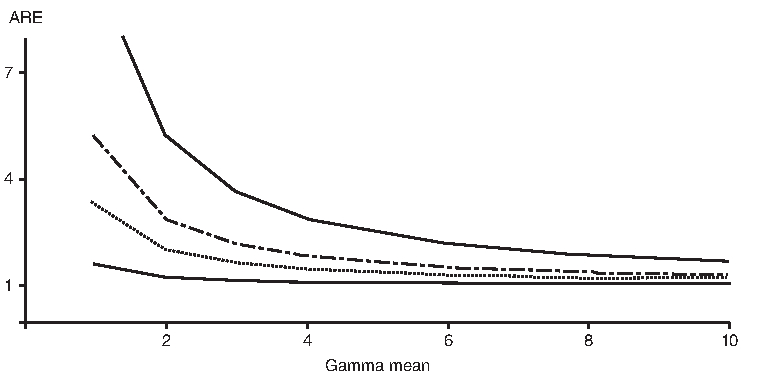
\includegraphics[width=.9\textwidth]{assets/chapter10/fig-10.1.1.pdf}
\caption{伽马均值的矩估计量与MLE的渐近相对效率. 四条曲线对应尺度参数值$(1,3,5,10)$，较高的曲线对应较大的尺度参数.}\label{fig:10.1.1}
\end{figure}\par
自助法由Efron于20世纪70年代末提出，最初的思想见Efron（\hyperref[bib:source106]{1979a}\hyperref[bib:source107]{b}），随后有专著\hyperref[bib:source108]{Efron（1982）}. 较新的思考与发展另见\hyperref[bib:source109]{Efron（1998）}.

先看一个其实并不需要自助法的简单例子.

\begin{example}[方差的自助法]\label{ex:10.1.19}\index{SI0095@非参数}\index{SI0913@重抽样}\index{SI0950@有放回}
在\autoref{ex:1.2.20}中，我们从四个数
$$2,4,9,12$$
中有放回地抽取四个数，计算所有可能的平均值. 这是最简单形式的自助法，有时称为非参数自助法（nonparametric bootstrap）. \autoref{fig:1.2.2}以直方图显示这些值.

所构造的是样本均值可能取值的重抽样. 已经看到，有$\binom{4+4-1}{4}=35$个不同的可能值，但它们并不等概率（所以不能视为随机样本）. $4^4=256$个（不全相异的）重抽样等可能，可以视为随机样本. 对第$i$个重抽样，令$\bar x_i^*$为其均值. 则样本均值$\bar X$的方差可估计为
\begin{equation}\label{eq:10.1.9}
\operatorname{Var}^*(\bar X)=\frac1{n^n-1}\sum_{i=1}^{n^n}(\bar x_i^*-\bar{\bar x}^{\,*})^2,
\end{equation}
其中$\bar{\bar x}^{\,*}=\frac1{n^n}\sum_{i=1}^{n^n}\bar x_i^*$是各个重抽样的均值. （通常以记号$*$表示自助法所得的、即重抽样所得的值.）

在本例中，自助法均值和方差分别为$\bar{\bar x}^{\,*}=6.75$和$\operatorname{Var}^*(\bar X)=3.94$. 事实表明，就均值和方差而言，自助法估计与通常估计几乎相同（见\autoref{exercise:10.13}）.
\end{example}

\sourcepageanchor{418}
我们已经看到如何计算自助法标准误，不过是在一个实际上不需要它的问题中. 自助法真正的优势在于，与Delta方法一样，方差公式\eqref{eq:10.1.9}几乎适用于任何估计量. 因此，对任意估计量$\hat\theta(\boldsymbol x)=\hat\theta$，可写为
\begin{equation}\label{eq:10.1.10}
\operatorname{Var}^*(\hat\theta)=\frac1{n^n-1}\sum_{i=1}^{n^n}(\hat\theta_i^*-\bar{\hat\theta}^{\,*})^2,
\end{equation}
其中$\hat\theta_i^*$是从第$i$个重抽样计算的估计量，$\bar{\hat\theta}^{\,*}=\frac1{n^n}\sum_{i=1}^{n^n}\hat\theta_i^*$是重抽样值的均值.

\begin{example}[二项方差的自助法]\label{ex:10.1.20}
在\autoref{ex:10.1.15}中，用Delta方法估计$\hat p(1-\hat p)$的方差. 对样本量$n$，也可将这个方差估计为
$$\operatorname{Var}^*(\hat p(1-\hat p))=\frac1{n^n-1}\sum_{i=1}^{n^n}\left((\hat p(1-\hat p))_i^*-\overline{\hat p(1-\hat p)}^{\,*}\right)^2.$$
\end{example}

但出现了新问题. 在\autoref{ex:10.1.19}中，$n=4$，自助法求和有256项. 对更典型的样本量，这个数会大到无法计算. （当$n>15$时，枚举全部可能的重抽样几乎不可能，至少对作者们如此.）不过，现在记起我们是统计学家：对重抽样再抽样即可.

因此，对样本$\boldsymbol x=(x_1,x_2,\ldots,x_n)$及估计$\hat\theta(x_1,x_2,\ldots,x_n)=\hat\theta$，选取$B$个重抽样（或自助样本，bootstrap samples），并计算
\begin{equation}\label{eq:10.1.11}\index{SI0913@重抽样}
\operatorname{Var}_B^*(\hat\theta)=\frac1{B-1}\sum_{i=1}^B(\hat\theta_i^*-\bar{\hat\theta}^{\,*})^2.
\end{equation}

\begin{example}[\autoref{ex:10.1.20}的结尾]\label{ex:10.1.21}
对样本量$n=24$，取$B=1{,}000$，计算$\hat p(1-\hat p)$的Delta方法方差估计和自助法方差估计. 当$\hat p\ne1/2$时，采用\autoref{ex:10.1.15}的一阶Delta方法方差估计；当$\hat p=1/2$时，采用\autoref{thm:5.5.26}的二阶方差估计（见\autoref{exercise:10.16}）. \autoref{tab:10.1.1}显示，在所有情形下，自助法方差估计都更接近真实方差，而Delta方法方差都低估了它. （这不应令人意外，因为\eqref{eq:10.1.7}表明Delta方法方差估计基于一个下界.）\footnote{译注：表中“真实值”与所述$n=24$二项模型不符. 按该模型对$Y=0,\ldots,24$逐项求和，$\operatorname{Var}[(Y/24)(1-Y/24)]$在$p=1/4,1/2,2/3$时约为$.001911,.000208,.001109$，并非表中的$.00484,.00531,.00519$. 原表及其比较结论保留；此核算仅针对表述的这三个参数值.}

\par\begin{table}[htbp]
\centering
\caption{$\hat p(1-\hat p)$的自助法（上行）与Delta方法（下行）方差. 当$\hat p=1/2$时使用二阶Delta方法（见\autoref{thm:5.5.26}）. 真实方差在假设$\hat p=p$下数值计算.}\label{tab:10.1.1}
\begin{tabular}{lrrr}\toprule
&$\hat p=1/4$&$\hat p=1/2$&$\hat p=2/3$\\\midrule
自助法&.00508&.00555&.00561\\
Delta方法&.00195&.00022&.00102\\\midrule
真实值&.00484&.00531&.00519\\\bottomrule
\end{tabular}
\end{table}\par

Delta方法是“一阶”近似，因为它基于泰勒级数展开的第一项. 当该项为零（例如$\hat p=1/2$）时，必须使用二阶Delta方法. 相比之下，自助法常有“二阶”准确性，能使展开中的不止第一项正确（见\hyperref[sec:10.6.3]{杂录10.6.3}）. 所以这里，自助法会自动修正$\hat p=1/2$的情形. （注意$24^{24}\approx1.33\times10^{13}$，这是极大的数，所以无法生成全部自助样本.）\footnote{译注：原文数值为$1.33\times10^{13}$，但$24^{24}\approx1.33\times10^{33}$. 保留原值；两者均支持这里无法枚举全部样本的结论.}
\end{example}

迄今讨论的自助法称为非参数自助法，因为没有假设总体pdf的函数形式.\index{SI0096@参数}\semanticindexanchor{96:418} 相比之下，也可以有参数自助法（parametric bootstrap）.

\sourcepageanchor{419}
假设样本$X_1,X_2,\ldots,X_n$来自pdf为$f(x\mid\theta)$的分布，其中$\theta$可以是参数向量. 可以用MLE $\hat\theta$估计$\theta$，并抽取样本
$$X_1^*,X_2^*,\ldots,X_n^*\sim f(x\mid\hat\theta).$$
若抽取$B$个这样的样本，就能用\eqref{eq:10.1.11}估计$\hat\theta$的方差. 注意，这些样本并非对数据的重抽样，而是从$f(x\mid\hat\theta)$实际抽出的随机样本；这个分布有时称为代入分布（plug-in distribution）.

\begin{example}[参数自助法]\label{ex:10.1.22}
假设有样本
$$-1.81,0.63,2.22,2.41,2.95,4.16,4.24,4.53,5.09,$$
其$\bar x=2.71$，$s^2=4.82$. 若假设基础分布为正态分布，则参数自助法会抽取样本
$$X_1^*,X_2^*,\ldots,X_n^*\sim\mathrm n(2.71,4.82).$$
基于$B=1000$个样本，算得$\operatorname{Var}_B^*(S^2)=4.33$. 根据正态理论，$S^2$的方差为$2(\sigma^2)^2/8$，可以用MLE $2(4.82)^2/8=5.81$估计它. 数据值模拟自方差为4的正态分布，因此这里参数自助法给出更好的估计. （在\autoref{ex:5.6.6}中，我们已经用现在所知的参数自助法估计过$S^2$的分布.）\footnote{译注：这里把以$s^2=4.82$代入的方差估计称为MLE；一般正态模型的方差MLE为$(n-1)s^2/n$，故该称呼与通常MLE定义不符. 原书数值与称呼均保留.}
\end{example}

现在有了一种计算标准误的通用方法，如何知道它是好方法呢？在\autoref{ex:10.1.21}中，它似乎优于Delta方法，而后者已知具有一些良好性质. 特别是，基于最大似然估计的Delta方法通常产生相合估计量. 对自助法能作相同的断言吗？

虽然无法十分一般地回答这个问题，但可以说，在许多情形下，自助法的确提供合理且相合的估计量.

为更精确，将计算自助法估计量的两个不同部分分开.
\begin{enumerate}[label=\alph*.]
\item\label{item:10.1.bootstrap.a} 证明当$B\to\infty$时，\eqref{eq:10.1.11}收敛到\eqref{eq:10.1.10}，即
$$\operatorname{Var}_B^*(\hat\theta)\xrightarrow{B\to\infty}\operatorname{Var}^*(\hat\theta).$$
\item\label{item:10.1.bootstrap.b}\index{SI0773@相合的自助法} 证明使用全部自助样本的估计量\eqref{eq:10.1.10}相合，即
$$\operatorname{Var}^*(\hat\theta)\xrightarrow{n\to\infty}\operatorname{Var}(\hat\theta).$$
\end{enumerate}
\hyperref[item:10.1.bootstrap.a]{(a)部分}可由大数定律建立（\autoref{exercise:10.15}）. 还应注意，\hyperref[item:10.1.bootstrap.a]{(a)部分}全部发生在样本内部. （\hyperref[bib:source199]{Lehmann，1999}，第6.5节把$\operatorname{Var}_B^*(\hat\theta)$称为近似器，而不是估计量.）

证明\hyperref[item:10.1.bootstrap.b]{(b)部分}稍微微妙一些，相合性正是在这里建立的. 独立同分布抽样时通常能够得到相合性，但在更一般的情形中未必如此（\hyperref[bib:source199]{Lehmann，1999}，第6.5节给出一个例子）. 关于相合性的更多细节（必然需要较高深的层次），见\hyperref[bib:source288]{Shao和Tu（1995}，第3.2.2节）或\hyperref[bib:source287]{Shao（1999}，第5.5.3节）.

\subsection{稳健性}\label{sec:10.2}
迄今为止，我们总是假设基础模型正确来评价估计量的表现. 在这个假设下，已经导出在某种意义下最优的估计量. 然而，若基础模型不正确，估计量的最优性就无法保证.

\sourcepageanchor{420}
我们无法防范所有可能的情形；而且，如果模型经过仔细考虑才确定，也不应有这种必要.\index{SI0813@稳健}\semanticindexanchor{813:420} 但我们可能关心与所假设模型的小幅或中等程度偏离. 这会引导我们考虑稳健估计量（robust estimators）. 这类估计量放弃在假设模型下的最优性，换取假设模型不是真实模型时的合理表现. 因此存在取舍，最优性与稳健性哪个更重要，最好视具体情形决定.

“稳健性”一词可以有多种解释；\hyperref[bib:source171]{Huber（1981}，第1.2节）的说法或许是最好的概括：
\begin{quote}
“……任何统计程序都应具有以下理想特征：
\begin{enumerate}[label=(\arabic*)]
\item\label{item:10.2.huber.1} 在假设模型下，应有相当好的（最优或近乎最优的）效率.
\item\label{item:10.2.huber.2} 它应当稳健，即模型假设的小幅偏离只应轻微损害表现……
\item\label{item:10.2.huber.3} 模型较大一些的偏离不应造成灾难.”
\end{enumerate}
\end{quote}
先看一些简单例子以更好地理解这些要求，然后再看更一般的稳健估计量和稳健性度量.

\subsubsection{均值与中位数}\label{sec:10.2.1}
样本均值是稳健估计量吗？这可能取决于如何精确地形式化稳健性的度量.

\begin{example}[样本均值的稳健性]\label{ex:10.2.1}
设$X_1,X_2,\ldots,X_n$独立同分布于$\mathrm n(\mu,\sigma^2)$. 已知$\bar X$的方差$\operatorname{Var}(\bar X)=\sigma^2/n$就是Cramér--Rao下界. 因而$\bar X$满足\hyperref[item:10.2.huber.1]{(1)}，在假设模型下达到最佳方差.

为研究\hyperref[item:10.2.huber.2]{(2)}，即$\bar X$在模型小幅偏离时的表现，先要明确这种偏离的含义. 通常的解释是采用$\delta$污染模型（$\delta$-contamination model），即对很小的$\delta$，假设观测到
$$X_i\sim\begin{cases}\mathrm n(\mu,\sigma^2),&\text{概率为$1-\delta$},\\f(x),&\text{概率为$\delta$},\end{cases}$$
其中$f(x)$是另一个分布.

假设取$f(x)$为任意均值为$\mu$、方差为$\tau^2$的密度. 则\footnote{译注：原文先说污染分布的均值为$\mu$，随后却使用未定义的$\theta$；若意指污染均值为$\theta$，独立样本均值的混合方差最后一项还应除以$n$. 此处原文与原式均保留.}
$$\operatorname{Var}(\bar X)=(1-\delta)\frac{\sigma^2}n+\delta\frac{\tau^2}n+\delta(1-\delta)(\theta-\mu)^2.$$
这看起来对$\bar X$相当有利，因为若$\theta\approx\mu$且$\sigma\approx\tau$，$\bar X$就接近最优. 不过，可以进一步扰动模型，使情况相当糟糕. 考虑$f(x)$为柯西pdf的情形，立即可得$\operatorname{Var}(\bar X)=\infty$. （细节见\autoref{exercise:10.18}，另一个情形见\autoref{exercise:10.19}.）
\end{example}

转向要求\hyperref[item:10.2.huber.3]{(3)}，我们问：若有一个异常偏离的观测，会发生什么？设想一组固定的样本值，然后考虑增大其中最大观测值的影响. 例如，假设$X_{(n)}=x$，其中$x\to\infty$. 这种观测的影响可被认为是“灾难性的”. 虽然$\bar X$的分布性质并未改变，观测值却会变得“毫无意义”. 这说明了崩溃值（breakdown value）的概念，该思想归于\hyperref[bib:source156]{Hampel（1974）}.

\begin{definition}\label{def:10.2.2}\index{SI0100@崩溃值}\index{SI0769@崩溃值}
设$X_{(1)}<\cdots<X_{(n)}$为容量$n$的有序样本，$T_n$为基于该样本的统计量. 若对每个$\varepsilon>0$，
$$\lim_{X_{(\{(1-b)n\})}\to\infty}T_n<\infty\quad\text{且}\quad
\lim_{X_{(\{(1-(b+\varepsilon))n\})}\to\infty}T_n=\infty,$$
则称$T_n$的崩溃值为$b$，$0\leq b\leq1$.
\end{definition}
（百分位数记号见\autoref{def:5.4.2}.）

\sourcepageanchor{421}
容易看出，$\bar X$的崩溃值是0，也就是说，将样本中任意比例的观测推向无穷，$\bar X$也随之趋于无穷. 与此形成鲜明对比，样本中位数不因样本值的这种变化而改变. 对极端观测的不敏感有时被视为样本中位数的优点，其崩溃值为50\%. （关于崩溃值的更多内容见\autoref{exercise:10.20}.）\footnote{译注：\autoref{def:10.2.2}的第一个极限在$b=0$时要求最大观测趋于无穷而统计量仍有限，与这里样本均值的说法在有限样本边界上不相容. 需明确崩溃比例的上确界或渐近约定，并限制$\varepsilon$以保证次序下标有效；原定义和结论照录，待核实.}

既然中位数比均值更稳健，我们可以问，改用更稳健的估计量是否会有所损失（当然一定会！）. 例如，在\autoref{ex:10.2.1}的简单正态模型中，如果模型真实，均值是最佳无偏估计量. 因此，在正态模型下（及其附近），均值是更好的估计量. 但关键问题是，在正态模型下均值究竟好多少. 若能回答，就可以有根据地选择估计量，并判断最优性和稳健性哪个准则更重要. 为在一定一般性下回答这个问题，使用渐近相对效率准则.

计算中位数相对于均值的ARE，首先必须建立中位数的渐近正态性，计算渐近分布的方差.

\begin{example}[中位数的渐近正态性]\label{ex:10.2.3}\index{SI0804@极限分布}
为求中位数的极限分布，采用与\autoref{thm:5.4.3}和\autoref{thm:5.4.4}证明相似的论证，即基于二项分布的论证.

设$X_1,X_2,\ldots,X_n$来自pdf为$f$、cdf为$F$（假设可微）的总体，且$P(X_i\leq\mu)=1/2$，所以$\mu$是总体中位数. 令$M_n$为样本中位数，考虑对某个$a$计算
$$\lim_{n\to\infty}P\bigl(\sqrt n(M_n-\mu)\leq a\bigr).$$
若定义随机变量$Y_i$为
$$Y_i=\begin{cases}1,&X_i\leq\mu+a/\sqrt n,\\0,&\text{其他},\end{cases}$$
则$Y_i$为成功概率$p_n=F(\mu+a/\sqrt n)$的伯努利随机变量. 为避免复杂情况，假设$n$为奇数，于是事件$\{M_n\leq\mu+a/\sqrt n\}$等价于$\{\sum_iY_i\geq(n+1)/2\}$.

作一些代数运算得到
$$P\bigl(\sqrt n(M_n-\mu)\leq a\bigr)=P\left(\frac{\sum_iY_i-np_n}{\sqrt{np_n(1-p_n)}}\geq\frac{(n+1)/2-np_n}{\sqrt{np_n(1-p_n)}}\right).$$
现在$p_n\to p=F(\mu)=1/2$，因此预期应用中心极限定理可证明$(\sum_iY_i-np_n)/\sqrt{np_n(1-p_n)}$依分布收敛到标准正态随机变量$Z$. 直接计算极限也可得到
$$\frac{(n+1)/2-np_n}{\sqrt{np_n(1-p_n)}}\longrightarrow-2aF'(\mu)=-2af(\mu).$$
综合起来，得到
$$P\bigl(\sqrt n(M_n-\mu)\leq a\bigr)\longrightarrow P(Z\geq-2af(\mu)),$$
因此$\sqrt n(M_n-\mu)$渐近正态，均值为0，方差为$1/[2f(\mu)]^2$. （细节见\autoref{exercise:10.22}；严格且更一般的推导见\hyperref[bib:source287]{Shao，1999}，第5.3节.）
\end{example}

\sourcepageanchor{422}
\begin{example}[中位数相对于均值的ARE]\label{ex:10.2.4}\index{SI0068@中位数相对于均值}
均值与中位数的渐近方差都有简单表达式，因此很快就能计算ARE. 这里考察三种对称分布的ARE，发现正如预期的那样，分布尾部越重，ARE越大. 也就是说，在重尾分布下中位数表现更好. 更多比较见\autoref{exercise:10.23}.
\end{example}
\par\begin{table}[htbp]
\centering\setcounter{table}{1}
\caption{中位数相对于均值的渐近相对效率}\label{tab:10.2.2}
\begin{tabular}{ccc}\toprule 正态分布&逻辑斯蒂分布&双指数分布\\\midrule .64&.82&2\\\bottomrule\end{tabular}
\end{table}\par

\subsubsection{\texorpdfstring{$M$}{M}估计量}\label{sec:10.2.2}\index{SI0816@M估计量}
许多估计量都是通过极小化某种准则得到的. 例如，若$X_1,X_2,\ldots,X_n$独立同分布于$f(x\mid\theta)$，可采用的估计量包括：均值，它极小化$\sum(x_i-a)^2$；中位数，它极小化$\sum|x_i-a|$；或MLE，它极大化$\prod_{i=1}^nf(x_i\mid\theta)$（或极小化负似然）. 作为系统获得稳健估计量的方法，可以尝试写出某种准则函数，使其极小值对应具有理想稳健性质的估计量.

为定义稳健准则，\hyperref[bib:source170]{Huber（1964）}考虑了均值与中位数之间的折中. 均值准则为平方，这赋予它敏感性，但在“尾部”，平方给予大观测过多的权重. 相比之下，中位数的绝对值准则不会过分加重大观测或小观测的权重. 折中方案是极小化准则函数
\begin{equation}\label{eq:10.2.1}
\sum_{i=1}^n\rho(x_i-a),
\end{equation}
其中$\rho$为
\begin{equation}\label{eq:10.2.2}\index{SI1043@调节参数}
\rho(x)=\begin{cases}\frac12x^2,&|x|\leq k,\\k|x|-\frac12k^2,&|x|\geq k.\end{cases}
\end{equation}
函数$\rho(x)$在$|x|\leq k$时类似$x^2$，在$|x|>k$时类似$|x|$. 此外，因为$\frac12k^2=k|k|-\frac12k^2$，该函数连续（\autoref{exercise:10.28}）. 常数$k$也称调节参数（tuning parameter），它控制两者的混合；$k$越小，得到的估计量越“类似中位数”.

\begin{example}[Huber估计量]\label{ex:10.2.5}\index{SI0814@Huber估计量}
以\eqref{eq:10.2.1}和\eqref{eq:10.2.2}的极小化点定义的估计量称为Huber估计量. 为了解它如何工作以及$k$的选择为何重要，考虑以下数据集，其中有八个标准正态偏差值和三个“离群值”：
$$\boldsymbol x=-1.28,-0.96,-0.46,-0.44,-0.26,-0.21,-0.063,0.39,3,6,9.$$
这些数据的均值为1.33，中位数为$-.21$. 随$k$变化，Huber估计值如\autoref{tab:10.2.3}所示. 可见当$k$增大时，Huber估计在中位数与均值之间变化，因此可以把增大$k$理解为降低对离群值的稳健性.

\par\begin{table}[htbp]\centering
\caption{Huber估计量}\label{tab:10.2.3}
\begin{tabular}{c|rrrrrrrrr}\toprule
$k$&0&1&2&3&4&5&6&8&10\\\midrule
估计值&$-.21$&.03&$-.04$&.29&.41&.52&.87&.97&1.33\\\bottomrule
\end{tabular}
\end{table}\par
\end{example}

极小化\eqref{eq:10.2.2}的估计量是Huber所研究估计量的特例. 对一般函数$\rho$，把极小化$\sum_i\rho(x_i-\theta)$的估计量称为$M$估计量（$M$-estimator），这个名称提醒我们它们属于最大似然型估计量（maximum-likelihood-type estimators）. 注意，若选择$\rho$为负对数似然$-l(\theta\mid\boldsymbol x)$，则$M$估计量就是通常的MLE.
\sourcepageanchor{423}
不过，若在选择待极小化的函数时更灵活，就能导出具有不同性质的估计量.

由于极小化函数通常通过求导数的零点来完成（在可求导时），定义$\psi=\rho'$，可见$M$估计量是方程
\begin{equation}\label{eq:10.2.3}
\sum_{i=1}^n\psi(x_i-\theta)=0
\end{equation}
的解.

将估计量刻画为方程的根，对研究其性质特别有用，因为似然估计中使用的论证可以推广.\index{SI1029@泰勒级数}\semanticindexanchor{1029:423} 特别参见\autoref{sec:10.1.2}，尤其是\autoref{thm:10.1.6}的证明. 假设$\rho(x)$对称，其导数$\psi(x)$单调递增（这保证\eqref{eq:10.2.3}的根是唯一极小值点）. 然后，像\autoref{thm:10.1.6}的证明一样，对$\phi$作泰勒展开如下：\footnote{译注：本段原文写$\phi$，但此前定义的是$\psi$；所引\autoref{thm:10.1.6}应核对为\autoref{thm:10.1.12}. 此外，对$\psi(x_i-\theta)$关于$\theta$展开，一阶项前应为负号；原文以下展开及整理后的负号均保留. 最后的方差因分母平方而不受此符号问题影响.}
$$\sum_{i=1}^n\psi(x_i-\theta)=\sum_{i=1}^n\psi(x_i-\theta_0)+(\theta-\theta_0)\sum_{i=1}^n\psi'(x_i-\theta_0)+\cdots,$$
其中$\theta_0$是真值，并忽略高阶项. 令$\hat\theta_M$为\eqref{eq:10.2.3}的解，代替$\theta$得到
$$0=\sum_{i=1}^n\psi(x_i-\theta_0)+(\hat\theta_M-\theta_0)\sum_{i=1}^n\psi'(x_i-\theta_0)+\cdots,$$
左侧为零是因为$\hat\theta_M$为解. 现在再次类似\autoref{thm:10.1.6}的证明，整理各项，除以$\sqrt n$，忽略余项，得到
$$\sqrt n(\hat\theta_M-\theta_0)=\frac{-\frac1{\sqrt n}\sum_{i=1}^n\psi(x_i-\theta_0)}{\frac1n\sum_{i=1}^n\psi'(x_i-\theta_0)}.$$
现假设$\theta_0$满足$E_{\theta_0}\psi(X-\theta_0)=0$（通常也将此作为$\theta_0$的定义）. 于是
\begin{equation}\label{eq:10.2.4}
-\frac1{\sqrt n}\sum_{i=1}^n\psi(X_i-\theta_0)
=\sqrt n\left[-\frac1n\sum_{i=1}^n\psi(X_i-\theta_0)\right]
\longrightarrow\mathrm n\bigl(0,E_{\theta_0}[\psi(X-\theta_0)]^2\bigr)
\end{equation}
依分布成立，而大数定律给出
\begin{equation}\label{eq:10.2.5}
\frac1n\sum_{i=1}^n\psi'(x_i-\theta_0)\longrightarrow E_{\theta_0}\psi'(X-\theta_0)
\end{equation}
依概率成立. 综合起来有
\begin{equation}\label{eq:10.2.6}\index{SI0815@极限分布}
\sqrt n(\hat\theta_M-\theta_0)\longrightarrow\mathrm n\left(0,\frac{E_{\theta_0}\psi(X-\theta_0)^2}{[E_{\theta_0}\psi'(X-\theta_0)]^2}\right).
\end{equation}

\begin{example}[Huber估计量的极限分布]\label{ex:10.2.6}
若$X_1,X_2,\ldots,X_n$独立同分布于pdf $f(x-\theta)$，其中$f$关于零对称，则对\eqref{eq:10.2.2}给出的$\rho$，有
\begin{equation}\label{eq:10.2.7}
\psi(x)=\begin{cases}x,&|x|\leq k,\\k,&x>k,\\-k,&x<-k,\end{cases}
\end{equation}
\sourcepageanchor{424}
所以\footnote{译注：按\eqref{eq:10.2.7}直接积分，下一式第一项应为正号，左右尾的系数应分别为$-k$与$k$；原文的负号及$\pm2k$与该定义不符. 对称性仍使两种写法均为零，原式保留.}
\begin{equation}\label{eq:10.2.8}
\begin{aligned}
E_\theta\psi(X-\theta)
&=-\int_{\theta-k}^{\theta+k}(x-\theta)f(x-\theta)\,dx\\
&\quad+2k\int_{-\infty}^{\theta-k}f(x-\theta)\,dx-2k\int_{\theta+k}^\infty f(x-\theta)\,dx\\
&=-\int_{-k}^kyf(y)\,dy+2k\int_{-\infty}^{-k}f(y)\,dy-2k\int_k^\infty f(y)\,dy=0,
\end{aligned}
\end{equation}
其中代入$y=x-\theta$. 由$f$的对称性，各积分相加为零. 因此Huber估计量具有正确的均值. （推广见\autoref{exercise:10.25}.）

为计算方差，需要$\psi'$的期望. 虽然$\psi$并非处处可微，但超出不可微点$x=\pm k$之后，$\psi'$为零. 因此只需处理$|x|\leq k$内的期望，有
$$\begin{aligned}
E_\theta\psi'(X-\theta)&=\int_{\theta-k}^{\theta+k}f(x-\theta)\,dx=P_0(|X|\leq k),\\
E_\theta[\psi(X-\theta)]^2
&=\int_{\theta-k}^{\theta+k}(x-\theta)^2f(x-\theta)\,dx\\
&\quad+k^2\int_{\theta+k}^\infty f(x-\theta)\,dx+k^2\int_{-\infty}^{\theta-k}f(x-\theta)\,dx\\
&=\int_{-k}^kx^2f(x)\,dx+2k^2\int_k^\infty f(x)\,dx.
\end{aligned}$$
因此，Huber估计量渐近正态，均值为$\theta$，渐近方差为
$$\frac{\int_{-k}^kx^2f(x)\,dx+k^2P_0(|X|>k)}{[P_0(|X|\leq k)]^2}.$$
\end{example}

像\autoref{ex:10.2.4}一样，现在考察多种分布下Huber估计量的ARE.

\begin{example}[Huber估计量的ARE]\label{ex:10.2.7}\index{SI0067@Huber估计量}
Huber估计量在某种意义上是均值与中位数的折中，因此考察它相对于这两个估计量的相对效率. 对正态分布和逻辑斯蒂分布，Huber估计量与均值表现相近，且优于中位数. 对双指数分布，它优于均值，但不如中位数. 回顾，均值是正态分布的MLE，中位数是双指数分布的MLE（因此预期ARE小于1）. 对这些分布，Huber估计量具有接近MLE的表现，同时在其他情形下似乎也保持合理表现.

\par\begin{table}[htbp]\centering
\caption{Huber估计量的渐近相对效率，$k=1.5$}\label{tab:10.2.4}
\begin{tabular}{l|ccc}\toprule
&正态分布&逻辑斯蒂分布&双指数分布\\\midrule
相对于均值&.96&1.08&1.37\\
相对于中位数&1.51&1.31&.68\\\bottomrule
\end{tabular}
\end{table}\par
\end{example}

可见，$M$估计量在稳健性与效率之间折中. 下面更仔细地看看，为获得稳健性，可能在效率方面放弃多少.

更仔细地考察\eqref{eq:10.2.6}中的渐近方差. 分母包含$E_{\theta_0}\psi'(X-\theta)$，可写为\footnote{译注：原文把$\psi'(x-\theta)$等同于$\partial\psi(x-\theta)/\partial\theta$；若撇号是对函数自变量求导，二者相差负号. 原式保留；下一页的乘积求导恒等式则显式处理了该负号.}
$$E_\theta\psi'(X-\theta)=\int\psi'(x-\theta)f(x-\theta)\,dx
=\int\left[\frac\partial{\partial\theta}\psi(x-\theta)\right]f(x-\theta)\,dx.$$

\sourcepageanchor{425}
现用乘积求导法则得到
$$\begin{aligned}
\frac d{d\theta}\int\psi(x-\theta)f(x-\theta)\,dx
&=\int\left[\frac d{d\theta}\psi(x-\theta)\right]f(x-\theta)\,dx\\
&\quad+\int\psi(x-\theta)\left[\frac d{d\theta}f(x-\theta)\right]\,dx.
\end{aligned}$$
若左侧为零——合理的$\psi$函数应当如此，仿照$l'$的行为——则有
$$\begin{aligned}
-\int\left[\frac d{d\theta}\psi(x-\theta)\right]f(x-\theta)\,dx
&=\int\psi(x-\theta)\left[\frac d{d\theta}f(x-\theta)\right]\,dx\\
&=\int\psi(x-\theta)\left[\frac d{d\theta}\log f(x-\theta)\right]f(x-\theta)\,dx,
\end{aligned}$$
其中利用了$\frac d{dy}g(y)/g(y)=\frac d{dy}\log g(y)$. 最后一个表达式可写为$E_\theta[\psi(X-\theta)l'(\theta\mid X)]$，其中$l(\theta\mid X)$是对数似然，从而得到恒等式
$$-E_\theta\left[\frac d{d\theta}\psi(X-\theta)\right]=E_\theta[\psi(X-\theta)l'(\theta\mid X)].$$
（取$\psi=l'$时，就得到我们希望读者已经熟悉的等式$-E_\theta[l''(\theta\mid X)]=E_\theta l'(\theta\mid X)^2$，见\autoref{lem:7.3.11}.）

现在比较$M$估计量与MLE的渐近方差就很简单. 回顾MLE $\hat\theta$的渐近方差为$E_\theta l'(\theta\mid X)^2$，因此\footnote{译注：原文此句将MLE渐近方差写为信息量；正确的通常形式是其倒数$1/E_\theta[l'(\theta\mid X)]^2$. 接下来的ARE公式与倒数形式一致. 原句保留.}
\begin{equation}\label{eq:10.2.9}
\operatorname{ARE}(\hat\theta_M,\hat\theta)=\frac{[E_\theta(\psi(X-\theta_0)l'(\theta\mid X)]^2}{E_\theta\psi(X-\theta)^2E_\theta l'(\theta\mid X)^2}\leq1,
\end{equation}
其中应用Cauchy--Schwarz不等式. 因此，$M$估计量的效率总低于MLE，且只有当$\psi$与$l'$成比例时才能达到相同效率（见\autoref{exercise:10.29}）.

本节并未试图将所有稳健估计量分类，而是满足于若干例子. 有许多优秀著作详细讨论稳健性；感兴趣的读者可阅读\hyperref[bib:source299]{Staudte和Sheather（1990）}或\hyperref[bib:source165]{Hettmansberger和McKean（1998）}\footnote{译注：原书正文将第一作者姓氏拼作Hettmansberger，书后对应条目[165]作Hettmansperger；正文拼写保留，链接至该条目.}.

\subsection{假设检验}\label{sec:10.3}
与\autoref{sec:10.1}一样，本节介绍几种在复杂问题中导出某些检验的方法. 所考虑的问题，是先前定义的最优检验不存在（例如不存在UMP无偏检验），或尚不知道最优检验的问题. 此时，导出任何合理的检验都可能有用. 以下两小节讨论似然比检验的大样本性质，以及其他近似大样本检验.

\subsubsection{似然比检验的渐近分布}\label{sec:10.3.1}
对复杂模型，构造检验最有用的方法之一是似然比法，因为它明确地定义检验统计量
$$\lambda(\boldsymbol x)=\frac{\sup_{\Theta_0}L(\theta\mid\boldsymbol x)}{\sup_\Theta L(\theta\mid\boldsymbol x)},$$
并明确给出拒绝域的形式$\{\boldsymbol x:\lambda(\boldsymbol x)\leq c\}$. 观测到数据$\boldsymbol X=\boldsymbol x$后，似然函数$L(\theta\mid\boldsymbol x)$就是变量$\theta$的完全确定的函数.
\sourcepageanchor{426}
即使不能解析地求出$L(\theta\mid\boldsymbol x)$在$\Theta_0$和$\Theta$上的两个上确界，通常也能数值计算. 因此，即使没有定义$\lambda(\boldsymbol x)$的方便公式，也能对观测数据点求得检验统计量$\lambda(\boldsymbol x)$.

为定义水平$\alpha$的检验，必须选择常数$c$使
\begin{equation}\label{eq:10.3.1}
\sup_{\theta\in\Theta_0}P_\theta\bigl(\lambda(\boldsymbol X)\leq c\bigr)\leq\alpha.
\end{equation}
若不能导出$\lambda(\boldsymbol x)$的简单公式，似乎就无望求出$\lambda(\boldsymbol X)$的抽样分布，从而知道如何选$c$以保证\eqref{eq:10.3.1}. 但借助渐近理论，可以获得近似答案.

类似\autoref{thm:10.1.12}，有如下结果.

\begin{theorem}[LRT的渐近分布：简单$H_0$]\label{thm:10.3.1}
为检验$H_0:\theta=\theta_0$对$H_1:\theta\ne\theta_0$，假设$X_1,\ldots,X_n$独立同分布于$f(x\mid\theta)$，$\hat\theta$为$\theta$的MLE，且$f(x\mid\theta)$满足\hyperref[sec:10.6.2]{杂录10.6.2}中的正则条件. 则在$H_0$下，当$n\to\infty$时，
$$-2\log\lambda(\boldsymbol X)\longrightarrow\chi_1^2\quad\text{依分布},$$
其中$\chi_1^2$是自由度为1的卡方随机变量.
\end{theorem}
\begin{proof}
首先在$\hat\theta$处对$\log L(\theta\mid\boldsymbol x)=l(\theta\mid\boldsymbol x)$作泰勒展开，得到
$$l(\theta\mid\boldsymbol x)=l(\hat\theta\mid\boldsymbol x)+l'(\hat\theta\mid\boldsymbol x)(\theta-\hat\theta)+l''(\hat\theta\mid\boldsymbol x)\frac{(\theta-\hat\theta)^2}{2!}+\cdots.$$
现将$l(\theta_0\mid\boldsymbol x)$的展开式代入$-2\log\lambda\boldsymbol x=-2l(\theta_0\mid\boldsymbol x)+2l(\hat\theta\mid\boldsymbol x)$，得到\footnote{译注：原文下式把平方差除以$-l''$；由上面的泰勒展开应为$-l''(\hat\theta\mid\boldsymbol x)(\theta_0-\hat\theta)^2$，或除以观测信息量的倒数. 分子原文还写$\theta$而非$\theta_0$. 原式及随后“分母”一词保留.}
$$-2\log\lambda(\boldsymbol x)\approx\frac{(\theta-\hat\theta)^2}{-l''(\hat\theta\mid\boldsymbol x)},$$
其中使用$l'(\hat\theta\mid\boldsymbol x)=0$. 由于分母是观测信息量$\hat I_n(\hat\theta)$，且$\frac1n\hat I_n(\hat\theta)\to I(\theta_0)$，由\autoref{thm:10.1.12}和Slutsky定理（\autoref{thm:5.5.17}），得到$-2\log\lambda(\boldsymbol X)\to\chi_1^2$.
\end{proof}

\begin{example}[泊松LRT]\label{ex:10.3.2}
基于独立同分布于Poisson$(\lambda)$的观测$X_1,\ldots,X_n$，检验$H_0:\lambda=\lambda_0$对$H_1:\lambda\ne\lambda_0$，有
$$-2\log\lambda(\boldsymbol X)=-2\log\left(\frac{e^{-n\lambda_0}\lambda_0^{\sum x_i}}{e^{-n\hat\lambda}\hat\lambda^{\sum x_i}}\right)
=2n\bigl[(\lambda_0-\hat\lambda)-\hat\lambda\log(\lambda_0/\hat\lambda)\bigr],$$
其中$\hat\lambda=\sum x_i/n$是$\lambda$的MLE. 应用\autoref{thm:10.3.1}，当$-2\log\lambda(\boldsymbol x)>\chi_{1,\alpha}^2$时，在水平$\alpha$下拒绝$H_0$.

为了解渐近近似的准确程度，对检验统计量作一个小型模拟. 取$\lambda_0=5$、$n=25$，\autoref{fig:10.3.1}画出$-2\log\lambda(\boldsymbol x)$的10,000个值的直方图，以及$\chi_1^2$的pdf. 二者吻合似乎相当合理. 此外，\autoref{tab:10.3.5}比较模拟（精确）临界点与$\chi_1^2$（近似）临界点，显示它们非常接近.
\end{example}

\autoref{thm:10.3.1}可推广到原假设涉及参数向量的情形. 下面的推广不予证明，它至少对大样本保证\eqref{eq:10.3.1}成立. 完整讨论见\hyperref[bib:source311]{Stuart、Ord和Arnold（1999}，第22章）.

\sourcepageanchor{427}
\par\begin{figure}[htbp]\centering
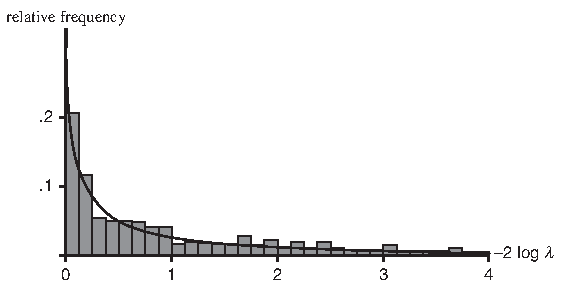
\includegraphics[width=.73\textwidth]{assets/chapter10/fig-10.3.1.pdf}
\caption{$-2\log\lambda(\boldsymbol x)$的10,000个值的直方图，以及$\chi_1^2$的pdf；$\lambda_0=5$，$n=25$.}\label{fig:10.3.1}
\end{figure}\par
\par\begin{table}[htbp]\centering\setcounter{table}{4}
\caption{泊松LRT统计量的模拟（精确）百分位数与近似百分位数}\label{tab:10.3.5}
\begin{tabular}{lrrrr}\toprule
百分位&.80&.90&.95&.99\\\midrule
模拟&1.630&2.726&3.744&6.304\\
$\chi^2$&1.642&2.706&3.841&6.635\\\bottomrule
\end{tabular}
\end{table}\par

\begin{theorem}\label{thm:10.3.3}\index{SI0632@渐近}
设$X_1,\ldots,X_n$是来自pdf或pmf $f(x\mid\theta)$的随机样本. 在\hyperref[sec:10.6.2]{杂录10.6.2}的正则条件下，若$\theta\in\Theta_0$，则统计量$-2\log\lambda(\boldsymbol X)$的分布随着样本量$n\to\infty$收敛到卡方分布. 极限分布的自由度，是$\theta\in\Theta_0$所规定的自由参数个数与$\theta\in\Theta$所规定的自由参数个数之差.
\end{theorem}

当$\lambda(\boldsymbol X)$较小时拒绝$H_0:\theta\in\Theta_0$，等价于当$-2\log\lambda(\boldsymbol X)$较大时拒绝. 因此，
$$\text{拒绝$H_0$当且仅当}\quad-2\log\lambda(\boldsymbol X)\geq\chi_{\nu,\alpha}^2,$$
其中$\nu$为\autoref{thm:10.3.3}规定的自由度. 若$\theta\in\Theta_0$且样本量大，第一类错误概率近似为$\alpha$.\index{SI0509@渐近}\semanticindexanchor{509:427} 这样，样本量大时\eqref{eq:10.3.1}近似满足，便定义了渐近大小为$\alpha$的检验. 注意，定理实际上仅意味着
$$\lim_{n\to\infty}P_\theta(\text{拒绝$H_0$})=\alpha\quad\text{对每个$\theta\in\Theta_0$},$$
并不意味着$\sup_{\theta\in\Theta_0}P_\theta(\text{拒绝$H_0$})$收敛到$\alpha$. 渐近大小为$\alpha$的检验通常如此.

检验统计量自由度的计算通常很直接. 最常见的是，$\Theta$可表示为$q$维欧氏空间的子集，并包含$\mathbb R^q$中的一个开子集；$\Theta_0$可表示为$p$维欧氏空间的子集，并包含$\mathbb R^p$中的一个开子集，其中$p<q$. 则$q-p=\nu$是检验统计量的自由度.

\begin{example}[多项LRT]\label{ex:10.3.4}\index{SI0636@多项}
设$\theta=(p_1,p_2,p_3,p_4,p_5)$，其中$p_j$非负且和为1. 假设$X_1,\ldots,X_n$为独立同分布的离散随机变量，$P_\theta(X_i=j)=p_j$，$j=1,\ldots,5$. 因此$X_i$的pmf为$f(j\mid\theta)=p_j$，似然函数为
$$L(\theta\mid\boldsymbol x)=\prod_{i=1}^nf(x_i\mid\theta)=p_1^{y_1}p_2^{y_2}p_3^{y_3}p_4^{y_4}p_5^{y_5},$$
\sourcepageanchor{428}
其中$y_j$为$x_1,\ldots,x_n$中等于$j$的个数. 考虑检验
$$H_0:p_1=p_2=p_3\text{且}p_4=p_5\qquad\text{对}\qquad H_1:H_0\text{不成立}.$$
完整参数空间$\Theta$实际上是四维集合. 因为$p_5=1-p_1-p_2-p_3-p_4$，只有四个自由参数. 参数集合由
$$\sum_{j=1}^4p_j\leq1\quad\text{且}\quad p_j\geq0,\quad j=1,\ldots,4$$
定义，是包含$\mathbb R^4$中开子集的$\mathbb R^4$子集. 因此$q=4$. $H_0$规定的集合只有一个自由参数，因为一旦固定$p_1$，$0\leq p_1\leq1/3$，则$p_2=p_3$必须等于$p_1$，而$p_4=p_5$必须等于$(1-3p_1)/2$. 因而$p=1$，自由度$\nu=4-1=3$.

计算$\lambda(\boldsymbol x)$，必须确定$\theta$在$\Theta_0$和$\Theta$下的MLE. 令
$$\frac\partial{\partial p_j}\log L(\theta\mid\boldsymbol x)=0\quad\text{对每个$j=1,\ldots,4$},$$
并利用$p_5=1-p_1-p_2-p_3-p_4$及$y_5=n-y_1-y_2-y_3-y_4$，可验证$p_j$在$\Theta$下的MLE为$\hat p_j=y_j/n$. 在$H_0$下，似然函数化为
$$L(\theta\mid\boldsymbol x)=p_1^{y_1+y_2+y_3}\left(\frac{1-3p_1}2\right)^{y_4+y_5}.$$
同样，以令导数为零的通常方法可得，$H_0$下$p_1$的MLE为$\hat p_{10}=(y_1+y_2+y_3)/(3n)$. 此时$\hat p_{10}=\hat p_{20}=\hat p_{30}$，且$\hat p_{40}=\hat p_{50}=(1-3\hat p_{10})/2$. 将这些值和$\hat p_j$代入$L(\theta\mid\boldsymbol x)$，合并相同指数的项，得到
$$\begin{aligned}
\lambda(\boldsymbol x)&=\left(\frac{y_1+y_2+y_3}{3y_1}\right)^{y_1}\left(\frac{y_1+y_2+y_3}{3y_2}\right)^{y_2}\left(\frac{y_1+y_2+y_3}{3y_3}\right)^{y_3}\\
&\quad\times\left(\frac{y_4+y_5}{2y_4}\right)^{y_4}\left(\frac{y_4+y_5}{2y_5}\right)^{y_5}.
\end{aligned}$$
因此检验统计量为
\begin{equation}\label{eq:10.3.2}
-2\log\lambda(\boldsymbol x)=2\sum_{i=1}^5y_i\log\left(\frac{y_i}{m_i}\right),
\end{equation}
其中$m_1=m_2=m_3=(y_1+y_2+y_3)/3$，$m_4=m_5=(y_4+y_5)/2$. 渐近大小为$\alpha$的检验在$-2\log\lambda(\boldsymbol x)\geq\chi_{3,\alpha}^2$时拒绝$H_0$. 本例属于广泛使用似然比检验渐近理论的一大类检验问题.
\end{example}

\subsubsection{其他大样本检验}\label{sec:10.3.2}\index{SI0204@依分布}
构造大样本检验统计量的另一常用方法，基于具有渐近正态分布的估计量. 假设要检验关于实值参数$\theta$的假设，$W_n=W(X_1,\ldots,X_n)$是通过某种方法导出的、基于容量$n$样本的$\theta$的点估计量. 例如，$W_n$可以是$\theta$的MLE. 基于正态近似的近似检验，可按如下方式论证. 若$\sigma_n^2$表示$W_n$的方差，且能用某种形式的中心极限定理证明，当$n\to\infty$时，$(W_n-\theta)/\sigma_n$依分布收敛到标准正态随机变量，那么就可以将$(W_n-\theta)/\sigma_n$与$\mathrm n(0,1)$分布比较，由此得到近似检验的基础.

当然，上段论证有许多细节需要验证，但这一思想确实适用于许多情形. 例如，若$W_n$为MLE，可以用\autoref{thm:10.1.12}来确立上述论证. 注意，$W_n$的分布以及可能的$\sigma_n$值依赖于$\theta$. 因而，更正式地说，对每个固定的$\theta\in\Theta$，若采用$W_n$相应的分布和$\sigma_n$相应的值，则$(W_n-\theta)/\sigma_n$收敛到标准正态分布.
\sourcepageanchor{429}
若对每个$n$，$\sigma_n$是可计算的常数（可依赖$\theta$，但不依赖其他未知参数），便可能导出基于$(W_n-\theta)/\sigma_n$的检验.

在一些情形中，$\sigma_n$还依赖未知参数.\index{SI0979@Slutsky定理}\semanticindexanchor{979:429} 此时寻找$\sigma_n$的估计$S_n$，使$\sigma_n/S_n$依概率收敛到1. 再由Slutsky定理（像\autoref{ex:5.5.18}一样），推出$(W_n-\theta)/S_n$也依分布收敛到标准正态分布. 大样本检验可据此构造.

假设要检验双侧假设$H_0:\theta=\theta_0$对$H_1:\theta\ne\theta_0$. 近似检验可基于统计量$Z_n=(W_n-\theta_0)/S_n$，当且仅当$Z_n<-z_{\alpha/2}$或$Z_n>z_{\alpha/2}$时拒绝$H_0$. 若$H_0$成立，则$\theta=\theta_0$，$Z_n$依分布收敛到$Z\sim\mathrm n(0,1)$. 因此，第一类错误概率
$$P_{\theta_0}(Z_n<-z_{\alpha/2}\text{或}Z_n>z_{\alpha/2})\longrightarrow P(Z<-z_{\alpha/2}\text{或}Z>z_{\alpha/2})=\alpha,$$
所以它是渐近大小为$\alpha$的检验.

现考虑备择参数值$\theta\ne\theta_0$. 可写为
\begin{equation}\label{eq:10.3.3}
Z_n=\frac{W_n-\theta_0}{S_n}=\frac{W_n-\theta}{S_n}+\frac{\theta-\theta_0}{S_n}.
\end{equation}
无论$\theta$取何值，都有$(W_n-\theta)/S_n\to\mathrm n(0,1)$. 通常还满足$n\to\infty$时$\sigma_n\to0$. （回顾$\sigma_n=\operatorname{Var}W_n$，而估计量通常随着$n\to\infty$越来越精确.）\footnote{译注：原文括号内写$\sigma_n=\operatorname{Var}W_n$，与前文$\sigma_n^2$为方差的定义不符；应为$\sigma_n^2=\operatorname{Var}W_n$. 原文保留.} 因而$S_n$依概率收敛到0，$(\theta-\theta_0)/S_n$根据$\theta-\theta_0$为正或负，分别依概率收敛到$+\infty$或$-\infty$. 于是$Z_n$也依概率收敛到$+\infty$或$-\infty$，且
$$P_\theta(\text{拒绝$H_0$})=P_\theta(Z_n<-z_{\alpha/2}\text{或}Z_n>z_{\alpha/2})\longrightarrow1,\qquad n\to\infty.$$
这样就能构造渐近大小为$\alpha$、渐近功效为1的检验.

若要检验单侧假设$H_0:\theta\leq\theta_0$对$H_1:\theta>\theta_0$，也能构造类似检验. 仍使用统计量$Z_n=(W_n-\theta_0)/S_n$，当且仅当$Z_n>z_\alpha$时拒绝$H_0$. 与上面类似的推理表明，检验的功效函数在$\theta<\theta_0$、$\theta=\theta_0$、$\theta>\theta_0$时分别收敛到0、$\alpha$、1. 所以该检验也有合理的渐近功效性质.

一般地，Wald检验（Wald test）是基于如下形式统计量的检验：
$$Z_n=\frac{W_n-\theta_0}{S_n},$$
其中$\theta_0$是参数$\theta$的假设值，$W_n$是$\theta$的估计量，$S_n$是$W_n$的标准误，即$W_n$标准差的估计. 若$W_n$是$\theta$的MLE，则如\autoref{sec:10.1.3}所述，$1/\sqrt{I(W_n)}$是合理的标准误. 也常使用$1/\sqrt{\hat I(W_n)}$，其中
$$\hat I(W_n)=-\left.\frac{\partial^2}{\partial\theta^2}\log L(\theta\mid\boldsymbol X)\right|_{\theta=W_n}$$
是观测信息量（见\eqref{eq:10.1.7}）.

\begin{example}[大样本二项检验]\label{ex:10.3.5}\index{SI0486@伯努利}
设$X_1,\ldots,X_n$为Bernoulli$(p)$总体的随机样本. 考虑检验$H_0:p\leq p_0$对$H_1:p>p_0$，其中$0<p_0<1$为指定值. 容量$n$样本中$p$的MLE为$\hat p_n=\sum_{i=1}^nX_i/n$. 因为$\hat p_n$就是样本均值，中心极限定理适用，且说明对任意$0<p<1$，$(\hat p_n-p)/\sigma_n$收敛到标准正态随机变量. 这里$\sigma_n=\sqrt{p(1-p)/n}$，依赖未知参数$p$.
\sourcepageanchor{430}
$\sigma_n$的合理估计为$S_n=\sqrt{\hat p_n(1-\hat p_n)/n}$，而且可以证明（\autoref{exercise:5.32}）$\sigma_n/S_n$依概率收敛到1. 因而，对任意$0<p<1$，
$$\frac{\hat p_n-p}{\sqrt{\hat p_n(1-\hat p_n)/n}}\longrightarrow\mathrm n(0,1).$$
将$p$替换为$p_0$，即定义了Wald检验统计量$Z_n$；大样本Wald检验在$Z_n>z_\alpha$时拒绝$H_0$. 作为$\sigma_n$的另一种估计，容易验证$1/I(\hat p_n)=\hat p_n(1-\hat p_n)/n$. 所以用信息量导出$\hat p_n$的标准误，也得到相同统计量$Z_n$.

若要检验双侧假设$H_0:p=p_0$对$H_1:p\ne p_0$，其中$0<p_0<1$为指定值，上述策略仍适用. 但此时还有另一种近似检验. 由中心极限定理，对任意$0<p<1$，
$$\frac{\hat p_n-p}{\sqrt{p(1-p)/n}}\longrightarrow\mathrm n(0,1).$$
因此，若原假设成立，统计量
\begin{equation}\label{eq:10.3.4}
Z'_n=\frac{\hat p_n-p_0}{\sqrt{p_0(1-p_0)/n}}\sim\mathrm n(0,1)\qquad\text{（近似地）}.
\end{equation}
近似水平$\alpha$的检验在$|Z'_n|>z_{\alpha/2}$时拒绝$H_0$.

当两个检验均适用时，例如检验$H_0:p=p_0$时，并不清楚应优先选择哪个. 它们的（实际而非近似）功效函数彼此交叉，所以每个检验都在参数空间的某一部分更有功效. （\hyperref[bib:source139]{Ghosh，1979}，对这个问题提供了一些见解. \hyperref[bib:source254]{Robbins，1977}，以及\hyperref[bib:source105]{Eberhardt和Fligner，1977}，讨论了相关的双样本二项问题争论. \autoref{exercise:10.31}给出该问题的两个不同检验统计量.）

当然，比较功效函数时会受到一个事实的干扰：这些是近似检验，不一定保持水平$\alpha$. 连续性校正（\autoref{ex:3.3.2}）有助于解决这个问题. 许多情形下，使用连续性校正的近似程序是保守的，即保持其名义$\alpha$水平（见\autoref{ex:10.4.6}）.
\end{example}

\eqref{eq:10.3.4}是另一种有用的大样本检验——得分检验（score test）——的特例. 定义得分统计量为
$$S(\theta)=\frac\partial{\partial\theta}\log f(\boldsymbol X\mid\theta)=\frac\partial{\partial\theta}\log L(\theta\mid\boldsymbol X).$$
由\eqref{eq:7.3.8}，对所有$\theta$，$E_\theta S(\theta)=0$. 特别地，若检验$H_0:\theta=\theta_0$且$H_0$成立，则$S(\theta_0)$均值为零. 此外，由\eqref{eq:7.3.10}，
$$\operatorname{Var}_\theta S(\theta)=E_\theta\left(\left(\frac\partial{\partial\theta}\log L(\theta\mid\boldsymbol X)\right)^2\right)
=-E_\theta\left(\frac{\partial^2}{\partial\theta^2}\log L(\theta\mid\boldsymbol X)\right)=I(\theta);$$
信息量就是得分统计量的方差. 得分检验的检验统计量为
$$Z_S=S(\theta_0)/\sqrt{I(\theta_0)}.$$
若$H_0$成立，$Z_S$均值为0、方差为1. 由\autoref{thm:10.1.12}，在$H_0$成立时，$Z_S$收敛到标准正态随机变量. 因此，近似水平$\alpha$的得分检验在$|Z_S|>z_{\alpha/2}$时拒绝$H_0$. 若$H_0$为复合假设，则在$Z_S$中用假定$H_0$成立时$\theta$的估计$\hat\theta_0$替代$\theta_0$. 若$\hat\theta_0$是受限MLE，受限极大化可借助拉格朗日乘子完成. 因而得分检验有时称为拉格朗日乘子检验（Lagrange multiplier test）.

\sourcepageanchor{431}
\begin{example}[二项得分检验]\label{ex:10.3.6}
再次考虑\autoref{ex:10.3.5}的伯努利模型，检验$H_0:p=p_0$对$H_1:p\ne p_0$. 直接计算得到
$$S(p)=\frac{\hat p_n-p}{p(1-p)/n}\quad\text{且}\quad I(p)=\frac n{p(1-p)}.$$
所以得分统计量为
$$Z_S=\frac{S(p_0)}{\sqrt{I(p_0)}}=\frac{\hat p_n-p_0}{\sqrt{p_0(1-p_0)/n}},$$
与\eqref{eq:10.3.4}相同.
\end{example}

最后考虑的一类近似检验是稳健检验（robust tests，见\hyperref[sec:10.6.6]{杂录10.6.6}）. 在\autoref{sec:10.2}看到，若$X_1,X_2,\ldots,X_n$是来自位置族的独立同分布样本，$\hat\theta_M$为$M$估计量，则
\begin{equation}\label{eq:10.3.5}
\sqrt n(\hat\theta_M-\theta_0)\longrightarrow\mathrm n\bigl(0,\operatorname{Var}_{\theta_0}(\hat\theta_M)\bigr),
\end{equation}
其中$\operatorname{Var}_{\theta_0}(\hat\theta_M)=E_{\theta_0}\psi(X-\theta_0)^2/[E_{\theta_0}\psi'(X-\theta_0)]^2$为渐近方差. 因此，可以构造“广义”得分统计量
$$Z_{GS}=\sqrt n\frac{\hat\theta_M-\theta_0}{\sqrt{\operatorname{Var}_{\theta_0}(\hat\theta_M)}},$$
或广义Wald统计量
$$Z_{GW}=\sqrt n\frac{\hat\theta_M-\theta_0}{\sqrt{\widehat{\operatorname{Var}}_{\theta_0}(\hat\theta_M)}},$$
其中$\widehat{\operatorname{Var}}_{\theta_0}(\hat\theta_M)$可为任意相合估计量. 例如，可以使用标准误的自助法估计，或直接将估计量代入\eqref{eq:10.2.6}而使用
\begin{equation}\label{eq:10.3.6}
\widehat{\operatorname{Var}}_1(\hat\theta_M)=\frac{\frac1n\sum_{i=1}^n[\psi(x_i-\hat\theta_M)]^2}{\left[\frac1n\sum_{i=1}^n\psi'(x_i-\hat\theta_M)\right]^2}.
\end{equation}
方差估计的选择可能很重要；相关指导见\hyperref[bib:source41]{Boos（1992）}或\hyperref[bib:source62]{Carroll等（1995}，附录A.3）.

\begin{example}[基于Huber估计量的检验]\label{ex:10.3.7}
若$X_1,X_2,\ldots,X_n$独立同分布于pdf $f(x-\theta)$，其中$f$关于零对称，则采用\eqref{eq:10.2.2}的$\rho$函数和\eqref{eq:10.2.7}的$\psi$函数的Huber $M$估计量，其渐近方差为
\begin{equation}\label{eq:10.3.7}
\frac{\int_{-k}^kx^2f(x)\,dx+k^2P_0(|X|>k)}{[P_0(|X|\leq k)]^2}.
\end{equation}
因此，根据$M$估计量的渐近正态性，例如可以在$|Z_{GS}|>z_{\alpha/2}$时拒绝$H_0$，以水平$\alpha$检验$H_0:\theta=\theta_0$对$H_1:\theta\ne\theta_0$. 为更切合实际，考察使用估计标准误的近似检验. 采用统计量$Z_{GW}$，但以\eqref{eq:10.3.7}为方差估计的基础，即\footnote{译注：下面分母原文为“1减去区间内比例”的平方；由\eqref{eq:10.3.7}应是区间内比例本身的平方，或将指标改为区间外. 原式保留.}
\begin{equation}\label{eq:10.3.8}
\widehat{\operatorname{Var}}_2(\hat\theta_M)=
\frac{\frac1n\sum_{i=1}^n(x_i-\hat\theta_M)^2I(|x_i-\hat\theta_M|<k)+k^2\left(\frac1n\sum_{i=1}^nI(|x_i-\hat\theta_M|>k)\right)}{\left(1-\frac1n\sum_{i=1}^nI(|x_i-\hat\theta_M|<k)\right)^2}.
\end{equation}
\sourcepageanchor{432}
另外加入一个“朴素”检验$Z_N$，使用简单的方差估计
\begin{equation}\label{eq:10.3.9}
\widehat{\operatorname{Var}}_3(\hat\theta_M)=\frac1n\sum_{i=1}^n(x_i-\hat\theta_M)^2.
\end{equation}
这些检验表现如何？解析评价很困难，但下面的小型模拟显示，$z_{\alpha/2}$临界值通常太小（忽略了方差估计的变动），实际大小一般大于名义大小. 不过，在一系列分布中的表现相当一致，双指数分布的情形最好. （最后这一点并不十分意外，因为Huber估计量对具有指数尾的分布享有一种最优性性质，见\hyperref[bib:source171]{Huber，1981}，第4章.）
\end{example}

\par\begin{table}[htbp]\centering
\caption{指定参数值处，基于$Z_{GW}$与$Z_N$的名义$\alpha=.1$检验的功效；样本量$n=15$，10,000次模拟.}\label{tab:10.3.6}
\small\begin{tabular}{lrrrrrrrr}\toprule
&\multicolumn{8}{c}{基础pdf}\\\cmidrule(lr){2-9}
&\multicolumn{2}{c}{正态}&\multicolumn{2}{c}{$t_5$}&\multicolumn{2}{c}{逻辑斯蒂}&\multicolumn{2}{c}{双指数}\\
&$Z_{GW}$&$Z_N$&$Z_{GW}$&$Z_N$&$Z_{GW}$&$Z_N$&$Z_{GW}$&$Z_N$\\\midrule
$\theta_0$&0.16&0.16&0.14&0.13&0.15&0.15&0.11&0.09\\
$\theta_0+.25\sigma$&0.27&0.29&0.29&0.27&0.27&0.27&0.31&0.26\\
$\theta_0+.5\sigma$&0.58&0.60&0.65&0.63&0.59&0.60&0.70&0.64\\
$\theta_0+.75\sigma$&0.85&0.87&0.89&0.89&0.85&0.87&0.92&0.90\\
$\theta_0+1\sigma$&0.96&0.97&0.98&0.97&0.96&0.97&0.98&0.98\\
$\theta_0+2\sigma$&1.&1.&1.&1.&1.&1.&1.&1.\\\bottomrule
\end{tabular}
\end{table}\par

\subsection{区间估计}\label{sec:10.4}
像前两节一样，现在探讨置信集的若干近似和渐近版本. 目的仍是说明一些在更复杂情形中有用、能够得到某种答案的方法. 这里所得的答案几乎肯定不是最好的，但也肯定不是最坏的. 不过，在许多情形下，它们是我们所能做到的最好结果.

与前面一样，从基于MLE的近似开始.

\subsubsection{近似最大似然区间}\label{sec:10.4.1}
由\autoref{sec:10.1.2}的讨论，使用\autoref{thm:10.1.12}，有一般方法求得MLE的渐近分布. 因而也有一般方法构造置信区间.

若$X_1,\ldots,X_n$独立同分布于$f(x\mid\theta)$，$\hat\theta$是$\theta$的MLE，则由\hyperref[eq:10.1.7]{(7.4.1)}，函数$h(\hat\theta)$的方差可近似为\footnote{译注：原文引用公式(7.4.1)，但与下式直接对应的是\eqref{eq:10.1.7}. 保留原引用，待对照作者勘误核实.}
$$\widehat{\operatorname{Var}}(h(\hat\theta)\mid\theta)\approx\frac{[h'(\theta)]^2|_{\theta=\hat\theta}}{-\frac{\partial^2}{\partial\theta^2}\log L(\theta\mid\boldsymbol x)|_{\theta=\hat\theta}}.$$

\sourcepageanchor{433}
现在，对固定但任意的$\theta$，关心
$$\frac{h(\hat\theta)-h(\theta)}{\sqrt{\widehat{\operatorname{Var}}(h(\hat\theta)\mid\theta)}}$$
的渐近分布. 由\autoref{thm:10.1.12}及Slutsky定理（\autoref{thm:5.5.17}；见\autoref{exercise:10.33}），
$$\frac{h(\hat\theta)-h(\theta)}{\sqrt{\widehat{\operatorname{Var}}(h(\hat\theta)\mid\theta)}}\longrightarrow\mathrm n(0,1),$$
从而给出近似置信区间
$$h(\hat\theta)-z_{\alpha/2}\sqrt{\widehat{\operatorname{Var}}(h(\hat\theta)\mid\theta)}\leq h(\theta)\leq h(\hat\theta)+z_{\alpha/2}\sqrt{\widehat{\operatorname{Var}}(h(\hat\theta)\mid\theta)}.$$

\begin{example}[续\autoref{ex:10.1.14}]\label{ex:10.4.1}\index{SI0138@二项}
设$X_1,\ldots,X_n$为Bernoulli$(p)$总体的随机样本. 已经看到，可以用MLE $\hat p/(1-\hat p)$估计优势比$p/(1-p)$，且这个估计的近似方差为
$$\widehat{\operatorname{Var}}\left(\frac{\hat p}{1-\hat p}\right)\approx\frac{\hat p}{n(1-\hat p)^3}.$$
因此，可以构造近似置信区间
$$\frac{\hat p}{1-\hat p}-z_{\alpha/2}\sqrt{\widehat{\operatorname{Var}}\left(\frac{\hat p}{1-\hat p}\right)}
\leq\frac p{1-p}\leq\frac{\hat p}{1-\hat p}+z_{\alpha/2}\sqrt{\widehat{\operatorname{Var}}\left(\frac{\hat p}{1-\hat p}\right)}.$$
\end{example}

一种限制较多的似然近似形式基于得分统计量（\autoref{sec:10.3.2}）；但在适用时，它能给出更好的区间. 随机量
\begin{equation}\label{eq:10.4.1}
Q(\boldsymbol X\mid\theta)=\frac{\frac\partial{\partial\theta}\log L(\theta\mid\boldsymbol X)}{\sqrt{-E_\theta\left(\frac{\partial^2}{\partial\theta^2}\log L(\theta\mid\boldsymbol X)\right)}}
\end{equation}
在$n\to\infty$时渐近服从$\mathrm n(0,1)$分布. 因此集合
\begin{equation}\label{eq:10.4.2}\index{SI0139@最大似然}
\{\theta:|Q(\boldsymbol x\mid\theta)|\leq z_{\alpha/2}\}
\end{equation}
是近似$1-\alpha$置信集. 注意，应用\autoref{sec:7.3.2}的结果，有
$$E_\theta(Q(\boldsymbol X\mid\theta))=\frac{E_\theta\left(\frac\partial{\partial\theta}\log L(\theta\mid\boldsymbol X)\right)}{\sqrt{-E_\theta\left(\frac{\partial^2}{\partial\theta^2}\log L(\theta\mid\boldsymbol X)\right)}}=0,$$
且
\begin{equation}\label{eq:10.4.3}
\operatorname{Var}_\theta(Q(\boldsymbol X\mid\theta))=\frac{\operatorname{Var}_\theta\left(\frac\partial{\partial\theta}\log L(\theta\mid\boldsymbol X)\right)}{-E_\theta\left(\frac{\partial^2}{\partial\theta^2}\log L(\theta\mid\boldsymbol X)\right)}=1.
\end{equation}
所以这个近似精确匹配$\mathrm n(0,1)$随机变量的前两阶矩. \hyperref[bib:source330]{Wilks（1938）}证明，这些区间具有渐近最优性：渐近地，它们是某类区间中最短的.

当然，这些区间并非完全一般，未必总能适用于函数$h(\theta)$. 必须能够把\eqref{eq:10.4.2}表示为$h(\theta)$的函数.

\sourcepageanchor{434}
\begin{example}[二项得分区间]\label{ex:10.4.2}
再次使用二项例子，若$Y=\sum_{i=1}^nX_i$，每个$X_i$都是独立的Bernoulli$(p)$随机变量，则有
$$\begin{aligned}
Q(Y\mid p)&=\frac{\frac\partial{\partial p}\log L(p\mid Y)}{\sqrt{-E_p\left(\frac{\partial^2}{\partial p^2}\log L(p\mid Y)\right)}}\\
&=\frac{\frac yp-\frac{n-y}{1-p}}{\sqrt{\frac n{p(1-p)}}}
=\frac{\hat p-p}{\sqrt{p(1-p)/n}},
\end{aligned}$$
其中$\hat p=y/n$. 利用\eqref{eq:10.4.2}，得到近似$1-\alpha$置信区间
\begin{equation}\label{eq:10.4.4}
\left\{p:\left|\frac{\hat p-p}{\sqrt{p(1-p)/n}}\right|\leq z_{\alpha/2}\right\}.
\end{equation}
这是反演得分统计量（\autoref{ex:10.3.6}）所得的区间. 计算它需要解一个关于$p$的二次方程，细节见\autoref{ex:10.4.6}.
\end{example}

在\autoref{sec:10.3}中，根据$-2\log\lambda(\boldsymbol X)$渐近服从卡方分布这一事实，导出了另一种似然检验. 这提示：若$X_1,\ldots,X_n$独立同分布于$f(x\mid\theta)$，$\hat\theta$是$\theta$的MLE，则集合
\begin{equation}\label{eq:10.4.5}
\left\{\theta:-2\log\left(\frac{L(\theta\mid\boldsymbol x)}{L(\hat\theta\mid\boldsymbol x)}\right)\leq\chi_{1,\alpha}^2\right\}
\end{equation}
是近似$1-\alpha$置信区间. 确实如此，这又给出了一个近似似然区间.

当然，\eqref{eq:10.4.5}就是最初通过反演LRT统计量导出的最高似然区域\eqref{eq:9.2.7}. 不过，现在有了自动赋予近似置信水平的方法.

\begin{example}[二项LRT区间]\label{ex:10.4.3}
若$Y=\sum_{i=1}^nX_i$，每个$X_i$都是独立的Bernoulli$(p)$随机变量，则近似$1-\alpha$置信集为
$$\left\{p:-2\log\left(\frac{p^y(1-p)^{n-y}}{\hat p^y(1-\hat p)^{n-y}}\right)\leq\chi_{1,\alpha}^2\right\}.$$
\autoref{ex:10.4.7}将比较这个置信集与基于得分检验和Wald检验的区间.
\end{example}

\subsubsection{其他大样本区间}\label{sec:10.4.2}
多数近似置信区间基于寻找近似（或渐近）枢轴量，或者反演近似水平$\alpha$的检验统计量. 若有任意统计量$W$、$V$与参数$\theta$，使$n\to\infty$时
$$\frac{W-\theta}V\longrightarrow\mathrm n(0,1),$$
则可以构造$\theta$的近似置信区间
$$W-z_{\alpha/2}V\leq\theta\leq W+z_{\alpha/2}V,$$
本质上是Wald型区间. 直接应用中心极限定理与Slutsky定理，通常就会给出近似置信区间. （注意，上一小节的近似最大似然区间均体现这一策略.）

\sourcepageanchor{435}
\begin{example}[近似区间]\label{ex:10.4.4}\index{SI0137@近似}
若$X_1,\ldots,X_n$独立同分布，均值为$\mu$、方差为$\sigma^2$，则由中心极限定理，
$$\frac{\bar X-\mu}{\sigma/\sqrt n}\longrightarrow\mathrm n(0,1).$$
此外，由Slutsky定理，若$S^2$依概率收敛到$\sigma^2$，则
$$\frac{\bar X-\mu}{S/\sqrt n}\longrightarrow\mathrm n(0,1),$$
给出近似$1-\alpha$置信区间
\begin{equation}\label{eq:10.4.6}
\bar x-z_{\alpha/2}s/\sqrt n\leq\mu\leq\bar x+z_{\alpha/2}s/\sqrt n.
\end{equation}
为了解近似有多好，对多种pdf进行小型模拟，计算近似区间的精确覆盖概率. 注意，因为区间基于枢轴量，覆盖概率不依赖参数值；它是常数，因此就是置信系数. \autoref{tab:10.4.7}显示，即使样本量小至$n=15$，枢轴置信区间也有合理表现，但显然达不到名义置信系数. 这无疑是由于使用$z_{\alpha/2}$临界值过于乐观，没有计入$S$的变动. 样本量增大时，近似将改善.

\par\begin{table}[htbp]\centering\setcounter{table}{6}
\caption{枢轴区间\eqref{eq:10.4.6}的置信系数，$n=15$，基于10,000次模拟}\label{tab:10.4.7}
\begin{tabular}{l|rrrr}\toprule
&\multicolumn{4}{c}{基础pdf}\\\cmidrule(lr){2-5}
名义水平&正态&$t_5$&逻辑斯蒂&双指数\\\midrule
$1-\alpha=.90$&0.879&0.864&0.880&0.876\\
$1-\alpha=.95$&0.931&0.924&0.931&0.933\\\bottomrule
\end{tabular}
\end{table}\par
\end{example}

上例无需指定抽样分布形式，就能得到近似置信区间. 当指定分布形式时，应能做得更好.

\begin{example}[近似泊松区间]\label{ex:10.4.5}\index{SI0141@泊松}
若$X_1,\ldots,X_n$独立同分布于Poisson$(\lambda)$，则知道
$$\frac{\bar X-\lambda}{S/\sqrt n}\longrightarrow\mathrm n(0,1).$$
不过，即使不是从泊松总体抽样，这也成立. 利用泊松假设，知道$\operatorname{Var}(X)=\lambda=EX$，且$\bar X$是$\lambda$的良好估计量（\autoref{sec:7}）. 因此利用泊松假设，还能由
$$\frac{\bar X-\lambda}{\sqrt{\bar X/n}}\longrightarrow\mathrm n(0,1)$$
得到近似置信区间，它是反演Wald检验所得的区间. 还可以用另一种方式利用泊松假设. 因为$\operatorname{Var}(X)=\lambda$，所以
$$\frac{\bar X-\lambda}{\sqrt{\lambda/n}}\longrightarrow\mathrm n(0,1),$$
由此得到与得分检验对应的区间，也就是\eqref{eq:10.4.2}的似然区间；按\hyperref[bib:source330]{Wilks（1938）}的结果，它是最优的（见\autoref{exercise:10.40}）.
\end{example}

\sourcepageanchor{436}
一般而言，合理的经验法则是，在近似中尽可能少用估计值、多用参数. 理由很简单：参数固定，不给近似引入额外变动，而每个统计量都会带来更多变动.

\begin{example}[再论二项得分区间]\label{ex:10.4.6}
对Bernoulli$(p)$总体的随机样本$X_1,\ldots,X_n$，在\autoref{ex:10.3.5}中看到，当$n\to\infty$时，
$$\frac{\hat p-p}{\sqrt{\hat p(1-\hat p)/n}}\quad\text{与}\quad\frac{\hat p-p}{\sqrt{p(1-p)/n}}$$
均依分布收敛到标准正态随机变量，其中$\hat p=\sum x_i/n$. 在\autoref{ex:10.3.5}中看到，可以基于任一近似建立检验，前者为Wald检验，后者为得分检验. 也知道可以用任一近似构造$p$的置信区间. 不过，得分检验近似使用较少的统计量和较多的参数值，会给出\autoref{ex:10.4.2}中的区间\eqref{eq:10.4.4}，它是渐近最优的. 即
$$\left\{p:\left|\frac{\hat p-p}{\sqrt{p(1-p)/n}}\right|\leq z_{\alpha/2}\right\}$$
是更好的近似区间.

这个区间的样子并不一目了然，但可以显式解出其取值集合. 两边平方并整理，就要寻找满足
$$\left\{p:(\hat p-p)^2\leq z_{\alpha/2}^2\frac{p(1-p)}n\right\}$$
的$p$值. 这是关于$p$的二次不等式，进一步整理可写成熟悉的形式：
$$\left\{p:\left(1+\frac{z_{\alpha/2}^2}n\right)p^2-\left(2\hat p+\frac{z_{\alpha/2}^2}n\right)p+\hat p^2\leq0\right\}.$$
由于二次项系数为正，抛物线开口向上，因此当$p$位于两个根之间时不等式成立. 两个根为
\begin{equation}\label{eq:10.4.7}
\frac{2\hat p+z_{\alpha/2}^2/n\ \pm\sqrt{(2\hat p+z_{\alpha/2}^2/n)^2-4\hat p^2(1+z_{\alpha/2}^2/n)}}{2(1+z_{\alpha/2}^2/n)},
\end{equation}
它们定义$p$的置信区间端点. 虽然根的表达式有些繁琐，这实际上是$p$的一个很好区间. 不过，使用连续性校正（\autoref{ex:3.3.2}）还可进一步改进. 为此，需要分别解两个二次不等式（见\autoref{exercise:10.45}）：
$$\begin{aligned}
\left|\frac{\hat p+\frac1{2n}-p}{\sqrt{p(1-p)/n}}\right|&\leq z_{\alpha/2},&&\text{（较大根为区间上端点）},\\
\left|\frac{\hat p-\frac1{2n}-p}{\sqrt{p(1-p)/n}}\right|&\leq z_{\alpha/2}.&&\text{（较小根为区间下端点）}.
\end{aligned}$$
在端点处有显然的修正：若$\sum x_i=0$，则区间下端点取0；若$\sum x_i=n$，则区间上端点取1. 一些良好近似见\hyperref[bib:source39]{Blyth（1986）}.
\end{example}

\sourcepageanchor{437}
现在已经看到二项比例的三个区间：基于Wald统计量、得分统计量的区间，以及\autoref{ex:10.4.3}的LRT区间. 通常最不优先选择Wald区间，不过比较三者仍很有意思.

\begin{example}[二项区间的比较]\label{ex:10.4.7}
对$Y=\sum_{i=1}^nX_i$，其中$X_1,\ldots,X_n$独立同分布于Bernoulli$(p)$总体，Wald区间为
\begin{equation}\label{eq:10.4.8}
\hat p-z_{\alpha/2}\sqrt{\frac{\hat p(1-\hat p)}n}\leq p\leq\hat p+z_{\alpha/2}\sqrt{\frac{\hat p(1-\hat p)}n}.
\end{equation}
带连续性校正的得分区间见\autoref{ex:10.4.6}，近似LRT见\autoref{ex:10.4.3}. 为比较它们，来看一个例子.

\par\begin{figure}[htbp]\centering
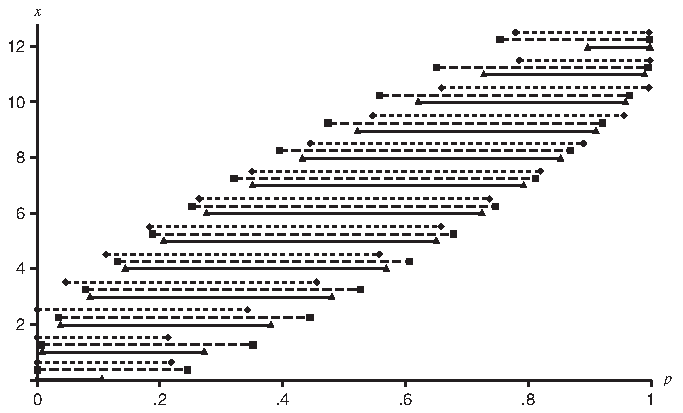
\includegraphics[width=.9\textwidth]{assets/chapter10/fig-10.4.1.pdf}
\caption{LRT程序（实线）、得分程序（长虚线）和修正Wald程序（短虚线）给出的二项比例区间.}\label{fig:10.4.1}
\end{figure}\par

对$n=12$，\autoref{fig:10.4.1}显示三种程序的区间实现值. LRT程序给出的区间最短，得分区间最长. 在这幅图中，对Wald区间作了两项修正. 首先，当$y=0$时，未修正区间为$(0,0)$，故将上端点改为$1-(\alpha/2)^{1/n}$；在$y=n$时对下端点作相似修正. 另外，Wald区间端点有时会超出$[0,1]$，这些部分已被截断.

得分区间较长，反映在其覆盖概率更高. 实际上，三者中只有得分区间保持覆盖概率在$.9$以上，因此只有它的置信系数为$.9$. LRT与Wald区间似乎太短，覆盖概率远低于$.9$，难以接受. 当然，随着$n$增大，它们的表现会改善. 其他选择见\hyperref[sec:9.5.2]{杂录9.5.2}.

所以，经过连续性校正的得分区间虽然更长，但似乎是小$n$时应选择的区间（另一种选择见\autoref{exercise:10.44}）. LRT和Wald程序在小$n$时产生的区间实在太短，Wald区间还存在端点问题.
\end{example}

像\autoref{sec:10.3.2}一样，简要考察基于稳健估计量的区间.

\begin{example}[基于Huber估计量的区间]\label{ex:10.4.8}
通过与\autoref{ex:10.3.7}类似的推导，可以构造基于Huber $M$估计量的渐近置信区间. 若$X_1,X_2,\ldots,X_n$独立同分布于pdf $f(x-\theta)$，其中$f$关于零对称，则$\theta$的近似区间为
\sourcepageanchor{438}
\par\begin{figure}[htbp]\centering
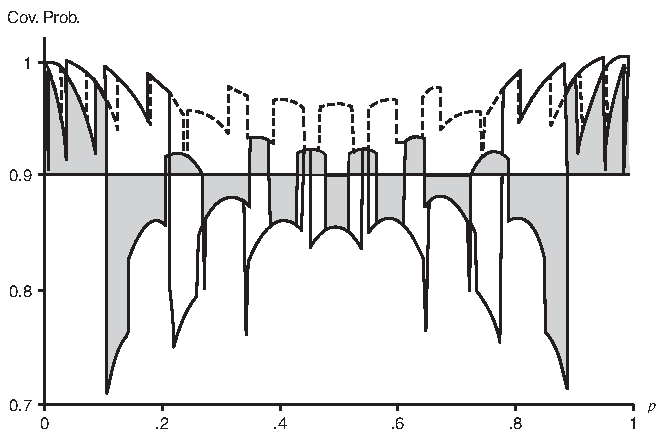
\includegraphics[width=.9\textwidth]{assets/chapter10/fig-10.4.2.pdf}
\caption{二项比例的名义$.9$置信程序的覆盖概率：LRT程序（细实线，灰色阴影）、得分程序（虚线）和修正Wald程序（粗实线）.}\label{fig:10.4.2}
\end{figure}\par
$$\hat\theta_M\pm z_{\alpha/2}\sqrt{\frac{\operatorname{Var}(\hat\theta_M)}n},$$
其中$\operatorname{Var}(\hat\theta_M)$由\eqref{eq:10.3.7}给出. 现在用估计\eqref{eq:10.3.8}与\eqref{eq:10.3.9}替换$\operatorname{Var}(\hat\theta_M)$，得到Wald型区间. 为评价它们，制作与\autoref{tab:10.4.7}相似的表. 有趣的是，除双指数分布外，\autoref{tab:10.4.8}中的区间表现都不如\autoref{tab:10.4.7}中基于通常均值与方差的区间. 对此没有很好的解释，只能再次归咎于$z_{\alpha/2}$临界值过于乐观.
\end{example}

\par\begin{table}[htbp]\centering
\caption{基于Huber $M$估计量、名义$1-\alpha=.9$的区间置信系数；$n=15$，基于10,000次模拟.}\label{tab:10.4.8}
\begin{tabular}{l|rrrr}\toprule
&\multicolumn{4}{c}{基础pdf}\\\cmidrule(lr){2-5}
名义水平&正态&$t_5$&逻辑斯蒂&双指数\\\midrule
方差估计\eqref{eq:10.3.8}&.844&.856&.855&.889\\
方差估计\eqref{eq:10.3.9}&.837&.867&.855&.910\\\bottomrule
\end{tabular}
\end{table}\par

迄今提到的近似都基于令$n\to\infty$. 不过，还有其他适合使用近似区间的情形. 在\autoref{ex:9.2.17}中，需要参数趋于无穷时的近似. 另一种情形见\autoref{ex:2.3.13}：对某些参数配置，泊松分布可以近似二项分布. 这提示，如果认为这种参数配置很可能成立，就能以泊松分布为基础构造近似二项区间. 本着这种想法，介绍下面这个略不寻常的例子.

\sourcepageanchor{439}
\begin{example}[负二项区间]\label{ex:10.4.9}\index{SI0140@负二项}
设$X_1,\ldots,X_n$独立同分布于negative binomial$(r,p)$. 假设$r$已知，希望得到$p$的置信区间. 利用$Y=\sum X_i\sim\operatorname{negative\ binomial}(nr,p)$，可以用多种方法构造区间. 利用二项分布与$F$分布关系的一个变形，可构造精确置信区间（\autoref{exercise:9.22}），也可使用正态近似（\autoref{exercise:10.41}）. 还有另一种近似，不依赖$n$大，而依赖$p$小.

\autoref{exercise:2.38}证明，当$p\to0$时，
$$2pY\longrightarrow\chi_{2nr}^2\quad\text{依分布}.$$
所以，对小$p$，$2pY$是枢轴量！据此可构造适用于小$p$的枢轴$1-\alpha$置信区间：
$$\left\{p:\frac{\chi_{2nr,1-\alpha/2}^2}{2y}\leq p\leq\frac{\chi_{2nr,\alpha/2}^2}{2y}\right\}.$$
细节见\autoref{exercise:10.47}.
\end{example}

\subsection{习题}\label{sec:10.5}

\begin{exercise}\label{exercise:10.1}
从pdf为
$$f(x\mid\theta)=\frac12(1+\theta x),\qquad-1<x<1,\quad-1<\theta<1$$
的总体中抽取随机样本$X_1,\ldots,X_n$. 求$\theta$的一个相合估计量，并证明其相合性.
\end{exercise}

\begin{exercise}\label{exercise:10.2}
证明\autoref{thm:10.1.5}.
\end{exercise}

\begin{exercise}\label{exercise:10.3}
从$\mathrm n(\theta,\theta)$总体中抽取随机样本$X_1,\ldots,X_n$，其中$\theta>0$.
\begin{enumerate}[label=(\alph*)]
\item 证明$\theta$的MLE $\hat\theta$是二次方程$\theta^2+\theta-W=0$的根，其中$W=(1/n)\sum_{i=1}^nX_i^2$，并确定哪个根等于MLE.
\item 用\autoref{sec:10.1.3}的技术求$\hat\theta$的近似方差.
\end{enumerate}
\end{exercise}

\begin{exercise}\label{exercise:10.4}
\autoref{exercise:7.19}模型的一个变形是令随机变量$Y_1,\ldots,Y_n$满足
$$Y_i=\beta X_i+\varepsilon_i,\qquad i=1,\ldots,n,$$
其中$X_1,\ldots,X_n$为独立的$\mathrm n(\mu,\tau^2)$随机变量，$\varepsilon_1,\ldots,\varepsilon_n$独立同分布于$\mathrm n(0,\sigma^2)$，且$X$与$\varepsilon$相互独立. 精确方差计算相当困难，因此可以采用近似. 用$\mu,\tau^2,\sigma^2$表示以下各量的近似均值与方差：
\begin{enumerate}[label=(\alph*)]
\item $\sum X_iY_i/\sum X_i^2$.
\item $\sum Y_i/\sum X_i$.
\item $\sum(Y_i/X_i)/n$.
\end{enumerate}
\end{exercise}

\begin{exercise}\label{exercise:10.5}
对\autoref{ex:10.1.8}的情形，令$T_n=\sqrt n/\bar X_n$，证明：
\begin{enumerate}[label=(\alph*)]
\item $\operatorname{Var}(T_n)=\infty$.
\item 若$\mu\ne0$且从样本空间删除区间$(-\delta,\delta)$，则$\operatorname{Var}(T_n)<\infty$.
\item 若$\mu\ne0$，区间$(-\delta,\delta)$的概率含量趋于0.\footnote{译注：此处需限制$\delta$相对$|\mu|$的大小；若区间包含$\mu$，则$\bar X_n$落在其中的概率反而趋于1. 原题条件照录，待核实所指样本空间及$\delta$约定.}
\end{enumerate}
\end{exercise}

\begin{exercise}\label{exercise:10.6}
对\autoref{ex:10.1.10}的情形，证明：
\begin{enumerate}[label=(\alph*)]
\item $EY_n=0$，且$\operatorname{Var}(Y_n)=p_n+(1-p_n)\sigma_n^2$；
\item $P(Y_n<a)\to P(Z<a)$，因而$Y_n\to\mathrm n(0,1)$（回顾$p_n\to1$、$\sigma_n\to\infty$且$(1-p_n)\sigma_n^2\to\infty$）.
\end{enumerate}
\end{exercise}

\begin{exercise}\label{exercise:10.7}
\autoref{thm:10.1.12}的证明说明了MLE $\hat\theta$是$\theta$的渐近有效估计量. 证明：若$\tau(\theta)$是$\theta$的连续函数，则$\tau(\hat\theta)$是$\tau(\theta)$的相合且渐近有效的估计量.
\end{exercise}

\sourcepageanchor{440}
\begin{exercise}\label{exercise:10.8}
通过建立\eqref{eq:10.1.6}中的两个收敛结果，完成\autoref{thm:10.1.6}的证明.\footnote{译注：原题引\autoref{thm:10.1.6}，但\eqref{eq:10.1.6}位于\autoref{thm:10.1.12}的证明中. 下列导数应在$\theta=\theta_0$处求值，原题未显式写出该代入.}
\begin{enumerate}[label=(\alph*)]
\item 证明
$$\frac1{\sqrt n}l'(\theta_0\mid\boldsymbol X)=\sqrt n\left[\frac1n\sum_iW_i\right],$$
其中$W_i=\frac{\frac d{d\theta}f(X_i\mid\theta)}{f(X_i\mid\theta)}$均值为0、方差为$I(\theta_0)$. 再用中心极限定理建立向$\mathrm n[0,I(\theta_0)]$的收敛.
\item 证明
$$-\frac1n l''(\theta_0\mid\boldsymbol X)=\frac1n\sum_iW_i^2-\frac1n\sum_i\frac{\frac{d^2}{d\theta^2}f(X_i\mid\theta)}{f(X_i\mid\theta)},$$
且第一部分均值为$I(\theta_0)$，第二部分均值为0. 应用弱大数定律.
\end{enumerate}
\end{exercise}

\begin{exercise}\label{exercise:10.9}
假设$X_1,\ldots,X_n$独立同分布于Poisson$(\lambda)$. 求以下各量的最佳无偏估计量：
\begin{enumerate}[label=(\alph*)]
\item\label{item:10.9.a} $e^{-\lambda}$，即$X=0$的概率.
\item\label{item:10.9.b} $\lambda e^{-\lambda}$，即$X=1$的概率.
\item 对\hyperref[item:10.9.a]{(a)}和\hyperref[item:10.9.b]{(b)}的最佳无偏估计量，计算相对于MLE的渐近相对效率. 你更倾向于哪些估计量？为什么？
\item 测量暴露于某种化合物的微生物突变率，可以对该化合物可能的致癌性进行初步检验. 实验者将化合物放入15个培养皿，记录到以下突变菌落数：
$$10,7,8,13,8,9,5,7,6,8,3,6,6,3,5.$$
估计没有突变菌落出现的概率$e^{-\lambda}$，以及出现一个突变菌落的概率$\lambda e^{-\lambda}$. 分别计算最佳无偏估计与MLE.
\end{enumerate}
\end{exercise}

\begin{exercise}\label{exercise:10.10}
继续\autoref{ex:10.1.14}的计算，那里考察了$p(1-p)$估计量的性质.\footnote{译注：直接讨论$p(1-p)$估计量的是\autoref{ex:10.1.15}，原题所引\autoref{ex:10.1.14}保留.}
\begin{enumerate}[label=(\alph*)]
\item 证明若$p\ne1/2$，MLE $\hat p(1-\hat p)$渐近有效.
\item 若$p=1/2$，用\autoref{thm:5.5.26}求$\hat p(1-\hat p)$的极限分布.
\item 计算$\operatorname{Var}[\hat p(1-\hat p)]$的精确表达式. 近似失效的原因是否更清楚了？
\end{enumerate}
\end{exercise}

\begin{exercise}\label{exercise:10.11}
本题考察\autoref{ex:10.1.18}计算的若干细节与推广.
\begin{enumerate}[label=(\alph*)]
\item 复现\autoref{fig:10.1.1}，计算$\beta$已知时的ARE. （可沿用\autoref{ex:12.6.7}的计算，或自行编程.）
\item 验证，无论$\beta$已知还是未知，$\operatorname{ARE}(\bar X,\hat\mu)$的比较都相同.
\item 对$\mu$已知时$\beta$的估计，证明矩估计与最大似然估计相同. （使用$(\alpha,\beta)$参数化可能更容易.）
\item 对$\mu$未知时$\beta$的估计，矩估计与最大似然估计不同. 用渐近相对效率比较它们，并作出类似\autoref{fig:10.1.1}的图，不同曲线对应不同$\mu$值.
\end{enumerate}
\end{exercise}

\begin{exercise}\label{exercise:10.12}
验证\hyperref[sec:10.6.1]{杂录10.6.1}的超有效估计量$d_n$渐近正态，其方差在$\theta\ne0$时为$v(\theta)=1$，在$\theta=0$时为$v(\theta)=a^2$. （超有效估计量的更多内容见\hyperref[bib:source200]{Lehmann和Casella，1998}，第6.2节.）
\end{exercise}

\needspace{6\baselineskip}
\begin{exercise}\label{exercise:10.13}
参照\autoref{ex:10.1.19}：
\begin{enumerate}[label=(\alph*)]
\item 验证样本$2,4,9,12$的自助法均值和方差分别为6.75与3.94.
\item\label{item:10.13.b} 验证6.75是原样本的均值.
\item\label{item:10.13.c} 验证，当除以$n$而非$n-1$时，均值的自助法方差与均值方差的通常估计相同.
\item 说明如何利用$\binom{4+4-1}{4}=35$个不同的可能重抽样计算自助法均值和标准误.
\item 对一般样本$X_1,X_2,\ldots,X_n$证明\hyperref[item:10.13.b]{(b)}和\hyperref[item:10.13.c]{(c)}.
\end{enumerate}
\end{exercise}

\sourcepageanchor{441}
\begin{exercise}\label{exercise:10.14}
在下列各情形中考察参数与非参数自助法. 比较估计结果，讨论这些方法的优缺点.
\begin{enumerate}[label=(\alph*)]
\item 参照\autoref{ex:10.1.22}，用非参数自助法估计$S^2$的方差.
\item 在\autoref{ex:5.6.6}中，实质上已经对泊松样本的$S^2$分布进行了参数自助法. 使用非参数自助法给出该分布的另一幅直方图.
\item 在\autoref{ex:10.1.18}中考察了伽马均值的估计. 假设来自gamma$(\alpha,\beta)$分布的随机样本为
$$0.28,0.98,1.36,1.38,2.4,7.42.$$
使用最大似然法和自助法估计分布的均值与方差.
\end{enumerate}
\end{exercise}

\begin{exercise}\label{exercise:10.15}\leavevmode
\begin{enumerate}[label=(\alph*)]
\item 证明当$B\to\infty$时，\eqref{eq:10.1.11}中的$\operatorname{Var}_B^*(\hat\theta)$收敛到\eqref{eq:10.1.10}中的$\operatorname{Var}^*(\hat\theta)$.
\item 固定$B$，对$i=1,2,\ldots$，计算自助法方差$\operatorname{Var}_{B_i}^*(\hat\theta)$. 用大数定律证明当$m\to\infty$时，$(1/m)\sum_{i=1}^m\operatorname{Var}_{B_i}^*(\hat\theta)\to\operatorname{Var}^*(\hat\theta)$.
\end{enumerate}
\end{exercise}

\begin{exercise}\label{exercise:10.16}
对\autoref{ex:10.1.21}的情形，若观测到$\hat p=1/2$，可以使用\autoref{thm:5.5.26}的方差估计. 证明这个方差估计等于$2[\operatorname{Var}(\hat p)]^2$.\footnote{译注：\hyperref[itm:exercise:10.16:a]{(a)}的$.00007$对应一阶Delta近似，而非题干所列二阶形式；\hyperref[itm:exercise:10.16:b]{(b)}的$.00529$也与$n=24,p=11/24$下对二项概率逐项求和所得方差（约$.000271$）不符. 原题数值保留，须核查原书的数值计算或统计量表述.}
\begin{enumerate}[label=(\alph*)]
\item\phantomsection\label{itm:exercise:10.16:a} 若观测到$\hat p=11/24$，验证此方差估计为$.00007$.
\item\phantomsection\label{itm:exercise:10.16:b} 使用模拟，计算$n=24$且$p=11/24$时$\hat p(1-\hat p)$的“精确方差”. 验证它等于$.00529$.
\item 你认为Delta方法在此情形下为何如此差？二阶Delta方法会更好吗？自助法估计又如何？
\end{enumerate}
\end{exercise}

\begin{exercise}\label{exercise:10.17}
\hyperref[bib:source108]{Efron（1982）}分析法学院录取数据，考察LSAT（法学院入学考试，Law School Admission Test）与第一年GPA（平均绩点，Grade Point Average）之间的相关性. 对15所法学院中的每所，得到一对数据（平均LSAT，平均GPA）.\footnote{译注：原表第三对数据写$(5.58,2.81)$，第二行第一对写$(580.3.07)$，均照录；可能分别为$(558,2.81)$与$(580,3.07)$，需与数据来源核实. \hyperref[itm:exercise:10.17:c]{(c)}原文写GRE，但本题分析的是GPA；亦照录.}
\begin{center}\small
\begin{tabular}{ccccc}
$(576,3.39)$&$(635,3.30)$&$(5.58,2.81)$&$(578,3.03)$&$(666,3.44)$\\
$(580.3.07)$&$(555,3.00)$&$(661,3.43)$&$(651,3.36)$&$(605,3.13)$\\
$(653,3.12)$&$(575,2.74)$&$(545,2.76)$&$(572,2.88)$&$(594,2.96)$
\end{tabular}
\end{center}
\begin{enumerate}[label=(\alph*)]
\item 计算LSAT与GPA之间的相关系数.
\item 使用非参数自助法估计相关系数的标准差，取$B=1000$次重抽样，并画出其直方图.
\item\phantomsection\label{itm:exercise:10.17:c} 使用参数自助法估计相关系数的标准差. 假设(LSAT, GRE)服从二元正态分布，估计五个参数. 再从这个二元正态分布生成1,000个各含15对数据的样本.
\item\label{item:10.17.d}\index{SI0274@相关}\index{SI0775@极限分布} 若$(X,Y)$服从相关系数为$\rho$的二元正态分布，样本相关系数为$r$，则可用Delta方法证明
$$\sqrt n(r-\rho)\longrightarrow\mathrm n(0,(1-\rho^2)^2).$$
用此事实估计$r$的标准差. 它与自助法估计相比如何？画出$r$的近似pdf.
\item\label{item:10.17.e}\index{SI1039@Fisher的z变换} Fisher的$z$变换是相关系数的方差稳定变换（variance stabilizing transformation，见\autoref{exercise:11.4}）. 若$(X,Y)$服从相关系数为$\rho$的二元正态分布，样本相关系数为$r$，则
$$\frac12\left[\log\left(\frac{1+r}{1-r}\right)-\log\left(\frac{1+\rho}{1-\rho}\right)\right]$$
近似正态. 用此事实画出$r$的近似pdf.
\end{enumerate}
（建立\hyperref[item:10.17.d]{(d)}的正态性结果需要一些繁琐的矩阵计算，见\hyperref[bib:source200]{Lehmann和Casella，1998}，例6.5. \hyperref[item:10.17.e]{(e)}的$z$变换比\hyperref[item:10.17.d]{(d)}的Delta方法更快地收敛到正态分布. \hyperref[bib:source99]{Diaconis和Holmes，1994}，对此问题做了穷尽的自助法计算，枚举全部77,558,760个相关系数.）
\end{exercise}

\sourcepageanchor{442}
\begin{exercise}\label{exercise:10.18}
对\hyperref[ex:10.2.1]{习题10.2.1}的情形，即$X_1,X_2,\ldots,X_n$独立同分布，其中$X_i$以概率$1-\delta$服从$\mathrm n(\theta,\sigma^2)$，以概率$\delta$服从$f(x)$，而$f(x)$为任意均值$\mu$、方差$\tau^2$的密度，证明
$$\operatorname{Var}(\bar X)=(1-\delta)\frac{\sigma^2}n+\delta\frac{\tau^2}n+\frac{\delta(1-\delta)(\theta-\mu)^2}n.$$
并推出柯西pdf的污染总会导致无穷方差. （提示：将混合模型写成分层模型. 令$Y$以概率$1-\delta$为0、以概率$\delta$为1. 则$\operatorname{Var}(X_i)=E[\operatorname{Var}(X_i)\mid Y]+\operatorname{Var}(E[X_i\mid Y])$.）\footnote{译注：原题称“习题10.2.1”，对应正文实际为\autoref{ex:10.2.1}. 提示第一项条件位置原文如上，按全方差公式应为$E[\operatorname{Var}(X_i\mid Y)]$. 此处保留原文.}
\end{exercise}

\begin{exercise}\label{exercise:10.19}
基础假设还可能因抽样中的相关性而被违反，这会严重影响样本均值的性质. 假设在\hyperref[ex:10.2.1]{习题10.2.1}所讨论的情形中引入相关性，即观测$X_1,X_2,\ldots,X_n$，各$X_i\sim\mathrm n(\theta,\sigma^2)$，但不再独立.\footnote{译注：原题“习题10.2.1”应指\autoref{ex:10.2.1}. \hyperref[item:10.19.b]{(b)}方差式中括号内的加号与协方差求和不符，通常应为$n-(1-\rho^n)/(1-\rho)$；\hyperref[itm:exercise:10.19:c]{(c)}还需初始变量处于平稳分布，且与后续创新独立，才能得出所列相关式. 原题均保留.}
\begin{enumerate}[label=(\alph*)]
\item 对等相关情形，即$i\ne j$时$\operatorname{Corr}(X_i,X_j)=\rho$，证明
$$\operatorname{Var}(\bar X)=\frac{\sigma^2}n+\frac{n-1}n\rho\sigma^2,$$
因此$n\to\infty$时$\operatorname{Var}(\bar X)\not\to0$.
\item\label{item:10.19.b} 若沿时间（或距离）观测$X_i$，有时假设相关性随时间（或距离）减小，一个具体模型是$\operatorname{Corr}(X_i,X_j)=\rho^{|i-j|}$. 证明在这种情形下
$$\operatorname{Var}(\bar X)=\frac{\sigma^2}n+\frac{2\sigma^2}{n^2}\frac\rho{1-\rho}\left(n+\frac{1-\rho^n}{1-\rho}\right),$$
所以$n\to\infty$时$\operatorname{Var}(\bar X)\to0$. （相关性的另一影响见\hyperref[sec:5.8.2]{杂录5.8.2}.）
\item\phantomsection\label{itm:exercise:10.19:c}\index{SI0072@自回归模型} \hyperref[item:10.19.b]{(b)}的相关结构出现在自回归AR(1)模型（autoregressive AR(1) model）中，假设$X_{i+1}=\rho X_i+\delta_i$，其中$\delta_i$独立同分布于$\mathrm n(0,1)$. 若$|\rho|<1$，定义$\sigma^2=1/(1-\rho^2)$，证明$\operatorname{Corr}(X_1,X_i)=\rho^{i-1}$.
\end{enumerate}
\end{exercise}

\begin{exercise}\label{exercise:10.20}\index{SI0100@崩溃值}
参照关于崩溃值的\autoref{def:10.2.2}，证明：
\begin{enumerate}[label=(\alph*)]
\item 若$T_n=\bar X_n$为样本均值，证明$b=0$.
\item 若$T_n=M_n$为样本中位数，证明$b=.5$.

在敏感性方面介于均值与中位数之间的估计量是\index{SI0929@截尾}\semanticindexanchor{929:442}\index{SI1042@截尾均值}\semanticindexanchor{1042:442}$\alpha$截尾均值（$\alpha$-trimmed mean），$0<\alpha<1/2$，定义如下：删去最小的$\alpha n$个观测和最大的$\alpha n$个观测，取剩余观测的算术平均，得到$\bar X_n^\alpha$.
\item 若$T_n=\bar X_n^\alpha$为样本的$\alpha$截尾均值，$0<\alpha<1/2$，证明$0<b<1/2$.
\end{enumerate}
\end{exercise}

\begin{exercise}\label{exercise:10.21}\index{SI0805@中位数绝对偏差}
均值与中位数的崩溃表现也延续到对应的尺度估计量. 对样本$X_1,\allowbreak X_2,\allowbreak\ldots,\allowbreak X_n$：
\begin{enumerate}[label=(\alph*)]
\item 证明样本方差$S^2=\sum(X_i-\bar X)^2/(n-1)$的崩溃值为0.
\item 一种稳健替代量是中位数绝对偏差（median absolute deviation，MAD），即$|X_1-m|,|X_2-m|,\ldots,|X_n-m|$的中位数，其中$m$为样本中位数. 证明该估计量的崩溃值为50\%.
\end{enumerate}
\end{exercise}

\begin{exercise}\label{exercise:10.22}
本题考察\autoref{ex:10.2.3}的若干细节.
\begin{enumerate}[label=(\alph*)]
\item 验证若$n$为奇数，则
$$P\bigl(\sqrt n(M_n-\mu)\leq a\bigr)=P\left(\frac{\sum_iY_i-np_n}{\sqrt{np_n(1-p_n)}}\geq\frac{(n+1)/2-np_n}{\sqrt{np_n(1-p_n)}}\right).$$
\item 验证$p_n\to p=F(\mu)=1/2$，且
$$\frac{(n+1)/2-np_n}{\sqrt{np_n(1-p_n)}}\longrightarrow-2aF'(\mu)=-2af(\mu).$$
（提示：证明$[(n+1)/2-np_n]/\sqrt n$是导数的极限形式.）
\sourcepageanchor{443}
\item 解释如何从
$$P\bigl(\sqrt n(M_n-\mu)\leq a\bigr)\longrightarrow P(Z\geq-2af(\mu))$$
得到$\sqrt n(M_n-\mu)$渐近正态、均值为0、方差为$1/[2f(\mu)]^2$的结论.
\end{enumerate}
（注意，只有$p_n$不依赖$n$时，中心极限定理才可直接应用. 由于这里确实依赖$n$，要严格得出极限正态性还需更多工作. 完成这些工作后，结果与预期一致.）
\end{exercise}

\begin{exercise}\label{exercise:10.23}\index{SI0386@Tukey}\index{SI0916@Tukey模型}
本题进一步考察中位数相对于均值的ARE，即$\operatorname{ARE}(M_n,\bar X)$.
\begin{enumerate}[label=(\alph*)]
\item 验证\autoref{ex:10.2.4}给出的三个ARE.
\item 证明$\operatorname{ARE}(M_n,\bar X)$不受尺度变化影响，即基础pdf为$f(x)$还是$(1/\sigma)f(x/\sigma)$没有区别.
\item 当基础分布为自由度$\nu$的Student $t$分布时，对$\nu=3,5,10,25,50,\infty$计算$\operatorname{ARE}(M_n,\bar X)$. 关于ARE与分布尾部，你能得出什么结论？
\item 当基础pdf为Tukey模型
$$X\sim\begin{cases}\mathrm n(0,1),&\text{概率为$1-\delta$},\\\mathrm n(0,\sigma^2),&\text{概率为$\delta$},\end{cases}$$
时，计算$\operatorname{ARE}(M_n,\bar X)$. 对一系列$\delta$和$\sigma$计算ARE. 关于均值和中位数的相对表现，你能得出什么结论？
\end{enumerate}
\end{exercise}

\begin{exercise}\label{exercise:10.24}
假设$\theta_0$满足$E_{\theta_0}\psi(X-\theta_0)=0$，证明\eqref{eq:10.2.4}与\eqref{eq:10.2.5}蕴含\eqref{eq:10.2.6}.
\end{exercise}

\begin{exercise}\label{exercise:10.25}
若$f(x)$是关于0对称的pdf，$\rho$为对称函数，证明$\int\psi(x-\theta)f(x-\theta)\,dx=0$，其中$\psi=\rho'$. 再证明，这意味着若$X_1,X_2,\ldots,X_n$独立同分布于$f(x-\theta)$，$\hat\theta_M$为$\sum_i\rho(x_i-\theta)$的极小化点，则$\hat\theta_M$渐近正态，其均值等于$\theta$的真值.
\end{exercise}

\begin{exercise}\label{exercise:10.26}
考察\autoref{ex:10.2.6}计算的若干细节.
\begin{enumerate}[label=(\alph*)]
\item 验证$E_\theta\psi'(X-\theta)$与$E_\theta[\psi(X-\theta)]^2$的表达式，从而验证$\hat\theta_M$的方差公式.
\item 计算$\psi'$的期望时，注意到$\psi$并非处处可微，但可处理其中可微的部分. 另一种做法是注意$\psi$的期望可微，在\eqref{eq:10.2.5}中可以写为
$$\frac1n\sum_{i=1}^n\psi'(x_i-\theta_0)\longrightarrow\left.\frac d{d\theta_0}E_\theta\psi(X-\theta_0)\right|_{\theta_0=\theta}.$$
证明这与\eqref{eq:10.2.5}的极限相同.\footnote{译注：按函数自变量求导的撇号约定，右侧关于$\theta_0$的导数应带负号；这与\autoref{sec:10.2.2}的符号疑误相同. 原式保留.}
\end{enumerate}
\end{exercise}

\begin{exercise}\label{exercise:10.27}
对\autoref{ex:10.6.2}的情形：\footnote{译注：\hyperref[itm:exercise:10.27:b]{(b)}中的中位数分段式未单列中位数恰等于污染点$x$的中间情形；原式照录，待核实端点约定.}
\begin{enumerate}[label=(\alph*)]
\item 验证$IF(\bar X,x)=x-\mu$.
\item\phantomsection\label{itm:exercise:10.27:b} 对中位数，若$P(X\leq m)=1/2$，则$T(F)=m$，或$m=F^{-1}(1/2)$. 若$X\sim F_\delta$，证明
$$P(X\leq a)=\begin{cases}(1-\delta)F(a),&x>a,\\(1-\delta)F(a)+\delta,&\text{其他},\end{cases}$$
从而
$$T(F_\delta)=\begin{cases}F^{-1}\left(\dfrac1{2(1-\delta)}\right),&x>F^{-1}\left(\dfrac1{2(1-\delta)}\right),\\F^{-1}\left(\dfrac{1/2-\delta}{1-\delta}\right),&\text{其他}.
\end{cases}$$
\item 证明
$$\frac1\delta\left[F^{-1}\left(\frac1{2(1-\delta)}\right)-F^{-1}\left(\frac12\right)\right]\longrightarrow\frac1{2f(m)},$$
并完成计算$IF(M,x)$的论证.

（提示：写成$a_\delta=F^{-1}\left(\frac1{2(1-\delta)}\right)$，说明此极限为$a'_\delta|_{\delta=0}$. 后者可用隐函数求导及$(1-\delta)^{-1}=2F(a_\delta)$计算.）
\end{enumerate}
\end{exercise}

\sourcepageanchor{444}
\begin{exercise}\label{exercise:10.28}
证明：若$\rho$由\eqref{eq:10.2.2}定义，则$\rho$与$\rho'$均连续.
\end{exercise}

\begin{exercise}\label{exercise:10.29}\index{SI0794@渐近有效}
由\eqref{eq:10.2.9}，知道$M$估计量不可能比最大似然估计量更有效. 不过，也知道何时能同样有效.
\begin{enumerate}[label=(\alph*)]
\item 证明：若取$\psi(x-\theta)=cl'(\theta\mid x)$，其中$l$为对数似然，$c$为常数，则\eqref{eq:10.2.9}取等号.
\item 对下列各分布，验证对应的$\psi$函数给出渐近有效的$M$估计量.
\begin{enumerate}[label=(\roman*)]
\item 正态：$f(x)=e^{-x^2/2}/\sqrt{2\pi}$，$\psi(x)=x$.
\item 逻辑斯蒂：$f(x)=e^{-x}/(1+e^{-x})^2$，$\psi(x)=\tanh(x)$，其中$\tanh(x)$为双曲正切（hyperbolic tangent）.\footnote{译注：所列逻辑斯蒂密度的位置得分与$\tanh(x/2)$成比例，而非$\tanh(x)$. 此处原式保留.}
\item 柯西：$f(x)=[\pi(1+x^2)]^{-1}$，$\psi(x)=2x/(1+x^2)$.
\item 最少信息分布（least informative distribution）：
$$f(x)=\begin{cases}Ce^{-x^2/2},&|x|\leq c,\\Ce^{-c|x|+c^2/2},&|x|>c,\end{cases}$$
对应$\psi(x)=\max\{-c,\min(c,x)\}$，$C$与$c$为常数.
\end{enumerate}
\end{enumerate}
（更多细节见\hyperref[bib:source171]{Huber，1981}，第3.5节.）
\end{exercise}

\begin{exercise}\label{exercise:10.30}
对$M$估计量，$\psi$函数与崩溃值之间存在联系. 细节相当复杂（\hyperref[bib:source171]{Huber，1981}，第3.2节），但可以概括为：若$\psi$有界，则对应$M$估计量的崩溃值为
$$b^*=\frac\eta{1+\eta},\quad\text{其中}\quad\eta=\min\left\{-\frac{\psi(-\infty)}{\psi(\infty)},-\frac{\psi(\infty)}{\psi(-\infty)}\right\}.$$
\begin{enumerate}[label=(\alph*)]
\item 计算\autoref{exercise:10.29}中有效$M$估计量的崩溃值. 哪些既有效又稳健？
\item\label{item:10.30.b} 计算下列其他$M$估计量的崩溃值：
\begin{enumerate}[label=(\roman*)]
\item \eqref{eq:10.2.1}给出的Huber估计量.
\item Tukey双权函数（Tukey's biweight）：$|x|\leq c$时$\psi(x)=x(c^2-x^2)$，其他情形为0，其中$c$为常数.
\item Andrews正弦波（Andrew's sine wave）：$|x|\leq c\pi$时$\psi(x)=c\sin(x/c)$，其他情形为0.
\end{enumerate}
\item 当基础分布为(i)正态、(ii)双指数时，评价\hyperref[item:10.30.b]{(b)}中估计量相对于MLE的ARE.
\end{enumerate}
\end{exercise}

\begin{exercise}\label{exercise:10.31}\index{SI0106@独立性卡方检验}\index{SI0197@列联表}\index{SI0491@列联表}
从多个总体采集的二项数据常以列联表（contingency table）呈现. 对两个总体，表格可能如下：
\begin{center}
\begin{tabular}{lccr}
&\multicolumn{2}{c}{总体}&\\
&1&2&合计\\\cline{2-3}
成功&\multicolumn{1}{|c|}{$S_1$}&\multicolumn{1}{c|}{$S_2$}&$S=S_1+S_2$\\
失败&\multicolumn{1}{|c|}{$F_1$}&\multicolumn{1}{c|}{$F_2$}&$F=F_1+F_2$\\\cline{2-3}
合计&$n_1$&$n_2$&$n=n_1+n_2$
\end{tabular}
\end{center}
其中总体1为binomial$(n_1,p_1)$，有$S_1$次成功与$F_1$次失败；总体2为binomial$(n_2,p_2)$，有$S_2$次成功与$F_2$次失败. 通常感兴趣的假设为
$$H_0:p_1=p_2\qquad\text{对}\qquad H_1:p_1\ne p_2.$$
\begin{enumerate}[label=(\alph*)]
\item\label{item:10.31.a} 证明可以基于统计量
$$T=\frac{(\hat p_1-\hat p_2)^2}{\left(\frac1{n_1}+\frac1{n_2}\right)\bigl(\hat p(1-\hat p)\bigr)}$$
建立检验，其中$\hat p_1=S_1/n_1$、$\hat p_2=S_2/n_2$、$\hat p=(S_1+S_2)/(n_1+n_2)$. 再证明当$n_1,n_2\to\infty$时，$T$的分布趋于$\chi_1^2$. （这是称为独立性卡方检验，chi squared test of independence，的一类检验的特例.）
\sourcepageanchor{445}
\item 另一种衡量偏离$H_0$程度的方法是计算期望频数表（expected frequency table）. 以边际合计为条件，按照$H_0:p_1=p_2$填表，即
\begin{center}
\renewcommand{\arraystretch}{1.7}
\begin{tabular}{lccr}
&\multicolumn{2}{c}{期望频数}&\\
&1&2&合计\\\cline{2-3}
成功&\multicolumn{1}{|c|}{$\dfrac{n_1S}{n_1+n_2}$}&\multicolumn{1}{c|}{$\dfrac{n_2S}{n_1+n_2}$}&$S=S_1+S_2$\\\cline{2-3}
失败&\multicolumn{1}{|c|}{$\dfrac{n_1F}{n_1+n_2}$}&\multicolumn{1}{c|}{$\dfrac{n_2F}{n_1+n_2}$}&$F=F_1+F_2$\\\cline{2-3}
合计&$n_1$&$n_2$&$n=n_1+n_2$
\end{tabular}
\end{center}
利用期望频数表，逐个单元计算并求和，得到统计量$T^*$：
$$\begin{aligned}
T^*&=\sum\frac{(\text{观测值}-\text{期望值})^2}{\text{期望值}}\\
&=\frac{\left(S_1-\frac{n_1S}{n_1+n_2}\right)^2}{\frac{n_1S}{n_1+n_2}}+\cdots+\frac{\left(F_2-\frac{n_2F}{n_1+n_2}\right)^2}{\frac{n_2F}{n_1+n_2}}.
\end{aligned}$$
用代数方法证明$T^*=T$，从而$T^*$渐近服从卡方分布.
\item 另一个可用来检验$p_1$和$p_2$相等的统计量为
$$T^{**}=\frac{\hat p_1-\hat p_2}{\sqrt{\frac{\hat p_1(1-\hat p_1)}{n_1}+\frac{\hat p_2(1-\hat p_2)}{n_2}}}.$$
证明在$H_0$下，$T^{**}$渐近服从$\mathrm n(0,1)$，因此其平方渐近服从$\chi_1^2$. 再证明$(T^{**})^2\ne T^*$.
\item 在什么情况下，一个统计量优于另一个？
\item 19世纪后期，Joseph Lister进行了一项著名的医学实验. 当时手术相关死亡率很高，Lister猜想使用消毒剂石炭酸会有所帮助. 数年间，Lister完成75例使用或不使用石炭酸的截肢手术，数据如下：
\begin{center}
\begin{tabular}{llcc}
&&\multicolumn{2}{c}{是否使用石炭酸？}\\
&&是&否\\\cline{3-4}
患者是否存活？&是&\multicolumn{1}{|c|}{34}&\multicolumn{1}{c|}{19}\\\cline{3-4}
&否&\multicolumn{1}{|c|}{6}&\multicolumn{1}{c|}{16}\\\cline{3-4}
\end{tabular}
\end{center}
用这些数据检验使用石炭酸是否与患者死亡有关.
\end{enumerate}
\end{exercise}

\begin{exercise}\label{exercise:10.32}\index{SI0485@渐近}\index{SI0499@McNemar检验}\leavevmode
\begin{enumerate}[label=(\alph*)]
\item 设$(X_1,\ldots,X_n)\sim\operatorname{multinomial}(m,p_1,\ldots,p_n)$. 考虑检验$H_0:p_1=p_2$对$H_1:p_1\ne p_2$. 一个常用的检验称为McNemar检验（McNemar's Test），在
$$\frac{(X_1-X_2)^2}{X_1+X_2}>\chi_{1,\alpha}^2$$
时拒绝$H_0$. 证明这个检验统计量具有如下形式（如\autoref{exercise:10.31}）：
$$\sum_1^n\frac{(\text{观测值}-\text{期望值})^2}{\text{期望值}},$$
其中$X_i$是观测单元频数，期望单元频数是在$p_1=p_2$假设下$mp_i$的MLE.
\sourcepageanchor{446}
\item McNemar检验常用于以下类型的问题. 先问受试者赞成还是反对某个陈述，再让他们阅读与该陈述有关的信息，随后再次询问赞成还是反对. 各类别回答人数汇总于如下$2\times2$表：
\begin{center}
\begin{tabular}{llcc}
&&\multicolumn{2}{c}{之前}\\
&&赞成&反对\\\cline{3-4}
之后&赞成&\multicolumn{1}{|c|}{$X_3$}&\multicolumn{1}{c|}{$X_2$}\\\cline{3-4}
&反对&\multicolumn{1}{|c|}{$X_1$}&\multicolumn{1}{c|}{$X_4$}\\\cline{3-4}
\end{tabular}
\end{center}
假设$H_0:p_1=p_2$意味着，从赞成改为反对者的比例，与从反对改为赞成者的比例相同. 另一种可检验的假设是：最初赞成的人中改变意见的比例，与最初反对的人中改变意见的比例相同. 用条件概率表达这个假设，证明它不同于上述$H_0$. （此假设可用类似\autoref{exercise:10.31}的$\chi^2$检验检验.）
\end{enumerate}
\end{exercise}

\begin{exercise}\label{exercise:10.33}
补全\autoref{thm:10.3.1}中的空缺. 用\autoref{thm:10.1.12}及Slutsky定理（\autoref{thm:5.5.17}）证明$(\theta-\hat\theta)/\sqrt{-l''(\hat\theta\mid\boldsymbol x)}\to\mathrm n(0,1)$，从而$-2\log\lambda(\boldsymbol X)\to\chi_1^2$.\footnote{译注：原题除以观测信息量的平方根，与\autoref{thm:10.3.1}证明中的同一疑误相连；通常应乘以该平方根，或除以其倒数. 原式保留.}
\end{exercise}

\begin{exercise}\label{exercise:10.34}
检验$H_0:p=p_0$对$H_1:p\ne p_0$，假设观测到独立同分布于Bernoulli$(p)$的$X_1,\ldots,X_n$.
\begin{enumerate}[label=(\alph*)]
\item 导出$-2\log\lambda(\boldsymbol x)$的表达式，其中$\lambda(\boldsymbol x)$为LRT统计量.
\item 像\autoref{ex:10.3.2}一样，模拟$-2\log\lambda(\boldsymbol x)$的分布，与$\chi^2$近似比较.
\end{enumerate}
\end{exercise}

\begin{exercise}\label{exercise:10.35}
设$X_1,\ldots,X_n$为$\mathrm n(\mu,\sigma^2)$总体的随机样本.
\begin{enumerate}[label=(\alph*)]
\item 若$\mu$未知、$\sigma^2$已知，证明$Z=\sqrt n(\bar X-\mu_0)/\sigma$是检验$H_0:\mu=\mu_0$的Wald统计量.
\item 若$\sigma^2$未知、$\mu$已知，求检验$H_0:\sigma=\sigma_0$的Wald统计量.
\end{enumerate}
\end{exercise}

\begin{exercise}\label{exercise:10.36}
设$X_1,\ldots,X_n$为gamma$(\alpha,\beta)$总体的随机样本，假设$\alpha$已知、$\beta$未知. 考虑检验$H_0:\beta=\beta_0$.
\begin{enumerate}[label=(\alph*)]
\item $\beta$的MLE是什么？
\item\label{item:10.36.b} 导出检验$H_0$的Wald统计量，在统计量的分子与分母中都使用MLE.
\item 重做\hyperref[item:10.36.b]{(b)}，但在标准误中使用样本标准差.
\end{enumerate}
\end{exercise}

\begin{exercise}\label{exercise:10.37}
设$X_1,\ldots,X_n$为$\mathrm n(\mu,\sigma^2)$总体的随机样本.
\begin{enumerate}[label=(\alph*)]
\item 若$\mu$未知、$\sigma^2$已知，证明$Z=\sqrt n(\bar X-\mu_0)/\sigma$是检验$H_0:\mu=\mu_0$的得分统计量.
\item 若$\sigma^2$未知、$\mu$已知，求检验$H_0:\sigma=\sigma_0$的得分统计量.
\end{enumerate}
\end{exercise}

\begin{exercise}\label{exercise:10.38}
设$X_1,\ldots,X_n$为gamma$(\alpha,\beta)$总体的随机样本，假设$\alpha$已知、$\beta$未知. 考虑检验$H_0:\beta=\beta_0$，导出检验$H_0$的得分统计量.
\end{exercise}

\begin{exercise}\label{exercise:10.39}
扩展\autoref{ex:10.3.7}中的比较.
\begin{enumerate}[label=(\alph*)]
\item 另一种基于Huber $M$估计量的检验，可以使用\eqref{eq:10.3.6}的方差估计. 考察这种检验统计量的表现，评价它作为\eqref{eq:10.3.8}或\eqref{eq:10.3.9}替代量的优点（或不足）.
\item 另一种基于Huber $M$估计量的检验，可以使用自助法计算的方差. 考察这种检验统计量的表现.
\item $\hat\theta_M$的一个稳健竞争者是中位数. 考察基于中位数的位置参数检验的表现.
\end{enumerate}
\end{exercise}

\begin{exercise}\label{exercise:10.40}
在\autoref{ex:10.4.5}中看到，泊松假设结合中心极限定理，可以基于
$$\frac{\bar X-\lambda}{\sqrt{\lambda/n}}\longrightarrow\mathrm n(0,1)$$
构造近似区间.
\sourcepageanchor{447}
证明，根据\hyperref[bib:source330]{Wilks（1938）}，该近似最优. 即证明
$$\frac{\bar X-\lambda}{\sqrt{\lambda/n}}=\frac{\frac\partial{\partial\lambda}\log L(\lambda\mid\boldsymbol X)}{\sqrt{-E_\lambda\left(\frac{\partial^2}{\partial\lambda^2}\log L(\lambda\mid\boldsymbol X)\right)}}.$$
\end{exercise}

\begin{exercise}\label{exercise:10.41}
设$X_1,\ldots,X_n$独立同分布于negative binomial$(r,p)$. 希望为负二项分布参数构造近似置信区间.
\begin{enumerate}[label=(\alph*)]
\item 计算Wilks近似\eqref{eq:10.4.3}，说明如何用此表达式构造置信区间.
\item\label{item:10.41.b} 求负二项分布均值的一个近似$1-\alpha$置信区间. 说明如何在区间中加入连续性校正.
\item \autoref{exercise:9.23}的蚜虫数据也可以用负二项分布建模. 利用\hyperref[item:10.41.b]{(b)}的结果，对蚜虫数据构造近似90\%置信区间，与\autoref{exercise:9.23}基于泊松分布的区间比较.
\end{enumerate}
\end{exercise}

\begin{exercise}\label{exercise:10.42}
证明\eqref{eq:10.4.5}等价于最高似然区域\eqref{eq:9.2.7}，即对任意固定$\alpha$水平，它们产生相同置信集.
\end{exercise}

\begin{exercise}\label{exercise:10.43}
在\autoref{ex:10.4.7}中，对Wald区间作了两项修正.
\begin{enumerate}[label=(\alph*)]
\item\label{item:10.43.a} 当$y=0$时，将上端点改为$1-(\alpha/2)^{1/n}$；当$y=n$时，将下端点改为$(\alpha/2)^{1/n}$. 说明选取这些端点的理由. （提示：\autoref{sec:9.2.3}.）
\item 第二项修正是将所有区间截断在$[0,1]$内. 证明这个改变结合\hyperref[item:10.43.a]{(a)}的改变，改进了原Wald区间.
\end{enumerate}
\end{exercise}

\begin{exercise}\label{exercise:10.44}
\hyperref[bib:source3]{Agresti和Coull（1998）}“强烈推荐”二项参数的得分区间，但担心像\eqref{eq:10.4.7}这样的公式对初等统计课程而言有些令人生畏. 为以更简单公式产生合理的二项区间，他们建议对Wald区间作如下修正：增加两次成功与两次失败，再使用原Wald公式\eqref{eq:10.4.8}. 即用$\hat p=(y+2)/(n+4)$代替$\hat p=y/n$. 从长度与覆盖概率两方面，将此区间与二项得分区间比较. 你是否同意它是得分区间的合理替代？

（\hyperref[bib:source271]{Samuels和Lu，1992}，建议了另一种基于样本量的Wald区间修正.）
\end{exercise}

\begin{exercise}\label{exercise:10.45}
解出\autoref{ex:10.4.6}所给带连续性校正的近似二项置信区间端点. 证明该区间比不带连续性校正的对应区间更宽，且经过校正的区间具有一致更高的覆盖概率. （事实上，未校正区间的覆盖概率不能保持$1-\alpha$，会在一些参数值处低于此水平. 经过校正的区间则对所有参数值都保持大于$1-\alpha$的覆盖概率.）
\end{exercise}

\begin{exercise}\label{exercise:10.46}
扩展\autoref{ex:10.4.8}中的比较.
\begin{enumerate}[label=(\alph*)]
\item 制作类似\autoref{tab:10.4.8}的表，考察基于中位数的位置参数区间的稳健性. （基于均值的区间已在\autoref{tab:10.4.7}中完成.）
\item 另一种基于Huber $M$估计量的区间，可以使用自助法计算的方差. 考察这种区间的稳健性.
\end{enumerate}
\end{exercise}

\begin{exercise}\label{exercise:10.47}
设$X_1,\ldots,X_n$独立同分布于negative binomial$(r,p)$.
\begin{enumerate}[label=(\alph*)]
\item 补全\autoref{ex:10.4.9}的细节，即证明对小$p$，区间
$$\left\{p:\frac{\chi_{2nr,1-\alpha/2}^2}{2\sum x}\leq p\leq\frac{\chi_{2nr,\alpha/2}^2}{2\sum x}\right\}$$
是近似$1-\alpha$置信区间.
\item 说明如何选择端点以获得最短的$1-\alpha$区间.
\end{enumerate}
\end{exercise}

\begin{exercise}\label{exercise:10.48}
对Fieller置信集的情形（见\hyperref[sec:9.5.3]{杂录9.5.3}），即给定来自参数为$(\mu_X,\allowbreak\mu_Y,\allowbreak\sigma_X^2,\allowbreak\sigma_Y^2,\allowbreak\rho)$的二元正态分布的随机样本$(X_1,Y_1),\allowbreak\ldots,\allowbreak(X_n,Y_n)$，求$\theta=\mu_Y/\mu_X$的近似置信区间. 使用\autoref{ex:5.5.27}中的近似矩计算并应用中心极限定理.
\end{exercise}

\subsection{杂录}\label{sec:10.6}
\sourcepageanchor{448}
\subsubsection{超有效性}\label{sec:10.6.1}\index{SI1014@超效率}
虽然\autoref{thm:7.3.9}的Cramér--Rao下界确实是方差的下界，但\autoref{def:10.1.11}与\autoref{thm:10.1.6}中关于渐近方差的下界可以被突破. Hodges给出了一个胜过\autoref{def:10.1.11}下界的估计量例子（见\hyperref[bib:source194]{LeCam，1953）}.

若$X_1,\ldots,X_n$独立同分布于$\mathrm n(\theta,1)$，$\theta$的无偏估计量的Cramér--Rao下界为$v(\theta)=1/n$. 估计量
$$d_n=\begin{cases}\bar X,&|\bar X|\geq1/n^{1/4},\\a\bar X,&|\bar X|<1/n^{1/4},\end{cases}$$
满足
$$\sqrt n(d_n-\theta)\longrightarrow\mathrm n[0,v(\theta)]\quad\text{依分布},$$
其中$\theta\ne0$时$v(\theta)=1$，$\theta=0$时$v(\theta)=a^2$. 若$a<1$，则不等式\eqref{eq:7.2.5}在$\theta=0$处被违反.\footnote{译注：要保证$a^2<1$，需$|a|<1$，或事先限定$0\leq a<1$；原文仅写$a<1$. 此段所引\autoref{thm:10.1.6}应核对为\autoref{thm:10.1.12}，所引不等式(7.2.5)也需核对. 原文均保留.}

像$d_n$这样的估计量称为超有效估计量（superefficient estimator）. 虽然可以在一定一般性下构造它们，但它们更像理论上的奇特现象，而非实际关注的对象. 原因是，使方差低于下界的$\theta$值构成零概率集合，即Lebesgue测度为零的集合. 不过，超有效估计量的存在提醒我们，在建立估计量性质时，始终应仔细检查假设（在一般情况下也要谨慎！）.

\subsubsection{适当的正则条件}\label{sec:10.6.2}\index{SI0912@正则条件}
“在适当的正则条件下”这句话有些被滥用，因为只要假设足够多，大概就能证明想要的任何结论. 不过，“正则条件”通常十分技术性、相当乏味，而且大多数合理问题中通常都满足. 但它们不可避免，我们应该处理它们. 为完整起见，给出一组足以严格建立\autoref{thm:10.1.6}与\autoref{thm:10.1.12}的正则条件. 这些不是最一般的条件，但对许多应用已经足够一般（一个显著例外是MLE位于参数空间边界的情况）. 预先提醒，以下内容不适合畏难者；跳过也不会对理解造成太大损失.

这些条件主要涉及密度的可微性，以及交换微分与积分的能力（如\autoref{thm:7.3.9}的条件）. 更多细节与更一般的讨论，见\hyperref[bib:source311]{Stuart、Ord和Arnold（1999}，第18章）、\hyperref[bib:source120]{Ferguson（1996}，第4部分），或\hyperref[bib:source200]{Lehmann和Casella（1998}，第6.3节）.

以下四个假设足以证明\autoref{thm:10.1.6}，即MLE的相合性：
\begin{enumerate}[label=(A\arabic*)]
\item\label{item:10.6.A1} 观测$X_1,X_2,\ldots,X_n$，其中$X_i\sim f(x\mid\theta)$独立同分布.
\item\label{item:10.6.A2} 观测密度$f(x\mid\theta)$彼此不同，即若$\theta\ne\theta'$，则$f(x\mid\theta)\ne f(x\mid\theta')$.
\item\label{item:10.6.A3} 密度$f(x\mid\theta)$具有共同支撑集，且$f(x\mid\theta)$关于$\theta$可微.
\item\label{item:10.6.A4} 参数空间$\Omega$包含开集$\omega$，真实参数值$\theta_0$是其内点.
\end{enumerate}
以下两个假设与\hyperref[item:10.6.A1]{(A1)}至\hyperref[item:10.6.A4]{(A4)}一起，足以证明\autoref{thm:10.1.12}，即MLE的渐近正态性与有效性.
\begin{enumerate}[label=(A\arabic*),start=5]
\item\label{item:10.6.A5} 对每个$x\in\mathcal X$，密度$f(x\mid\theta)$关于$\theta$三次可微，三阶导数关于$\theta$连续，且$\int f(x\mid\theta)\,dx$可在积分号下对$\theta$求导三次.
\sourcepageanchor{449}
\item\label{item:10.6.A6} 对任意$\theta_0\in\Omega$，存在正数$c$与函数$M(x)$（二者均可依赖$\theta_0$），使
$$\left|\frac{\partial^3}{\partial\theta^3}\log f(x\mid\theta)\right|\leq M(x)\quad\text{对所有$x\in\mathcal X$、$\theta_0-c<\theta<\theta_0+c$},$$
且$E_{\theta_0}[M(X)]<\infty$.
\end{enumerate}

\subsubsection{再论自助法}\label{sec:10.6.3}
\paragraph{理论}
自助法背后的理论相当精深，以Edgeworth展开（Edgeworth expansions）为基础. 它们是在正态分布附近对分布函数进行的展开，其精神类似泰勒级数展开. 例如，若$X_1,X_2,\ldots,X_n$独立同分布，密度为$f$，均值和方差分别为$\mu$与$\sigma^2$，则$\sqrt n(\bar X-\mu)/\sigma$的cdf的一个Edgeworth展开为（\hyperref[bib:source154]{Hall，1992}，式2.17）
$$P\left(\frac{\sqrt n(\bar X-\mu)}\sigma\leq w\right)=\Phi(w)+\phi(w)\left[-\frac1{6\sqrt n}\kappa(w^2-1)+O\left(\frac1n\right)\right],$$
其中$\Phi$与$\phi$分别为标准正态分布函数与密度函数，$\kappa=E(X_1-\mu)^3$为偏度.\footnote{译注：对于此标准化后的展开，偏度通常应为$E[(X_1-\mu)^3]/\sigma^3$；原文定义缺少$\sigma^3$，除非另有$\sigma=1$的约定. 保留原式.} 展开的第一项是“通常”的正态近似；增加项数会提高展开的准确性.

自助法令人惊讶之处在于，在某些情形下，它会自动使展开的第二项正确（从而达到“二阶”准确性）. 并非所有情形都如此，但对枢轴量进行自助法就是其中一种. \hyperref[bib:source154]{Hall（1992）}全面讨论了自助法的Edgeworth理论，另见\hyperref[bib:source288]{Shao和Tu（1995）}.

\paragraph{实践}
我们仅用自助法计算过标准误，它还有许多用途，其中最流行的可能是构造置信区间. 此外，还有针对不同情形发展的许多自助法变体. 特别是，处理相依数据较为微妙. 关于自助法诸多用途及更多内容的入门介绍，见\hyperref[bib:source114]{Efron和Tibshirani（1993）}.

\paragraph{局限}
自助法或许是近年统计方法学中最重要的单项发展，但它也有局限，也有人持批评态度. 超出独立同分布抽样与枢轴量的情形，自助法就不那么自动化了，但仍可能极有用. 对这些问题的有趣讨论，见\hyperref[bib:source203]{LePage和Billard（1992）}或\hyperref[bib:source336]{Young（1994）}.

\subsubsection{影响函数}\label{sec:10.6.4}\index{SI0580@影响函数}
影响函数（influence function）是一种考虑分布性质的灾难性事件度量，也用于衡量异常观测的影响. 影响函数可以解释为导数，这还带来一些有趣的结果.

统计量的影响函数实际上用其总体对应量计算. 例如，样本均值的影响函数使用总体均值计算，因为它试图度量扰动总体的影响. 类似地，样本中位数的影响函数使用总体中位数计算. 为一致地处理这个思想，可以把估计量看成作用于cdf $F$或其样本对应量——经验cdf $F_n$（\autoref{def:1.5.1}）——的函数. 这种以其他函数为自变量的函数，称为泛函（functionals）.\index{SI0447@泛函}\semanticindexanchor{447:449}

\sourcepageanchor{450}
注意，对样本$X_1,X_2,\ldots,X_n$，知道样本等价于知道经验cdf $F_n$，因为$F_n$在每个$X_i$处跳跃$1/n$. 因此统计量$T=T(X_1,X_2,\ldots,X_n)$可等价写成$T(F_n)$，其总体对应量便可记为$T(F)$.

\begin{definition}\label{def:10.6.1}
对来自cdf为$F$的总体的样本$X_1,X_2,\ldots,X_n$，统计量$T=T(F_n)$在点$x$处的影响函数为
$$IF(T,x)=\lim_{\delta\to0}\frac1\delta[T(F_\delta)-T(F)],$$
其中，当
$$X\sim\begin{cases}F,&\text{概率为$1-\delta$},\\x,&\text{概率为$\delta$},\end{cases}$$
时，记$X\sim F_\delta$；即$F_\delta$是$F$与点$x$的混合.
\end{definition}

\begin{example}[均值与中位数的影响函数]\label{ex:10.6.2}\index{SI0798@影响函数}
假设总体具有连续cdf $F$与pdf $f$. 令$\mu$为总体均值，$\bar X$为样本均值，$T(\cdot)$为计算总体均值的泛函. 因此$T(F_n)=\bar X$，$T(F)=\mu$，且
$$T(F_\delta)=(1-\delta)\mu+\delta x,$$
所以$IF(\bar X,x)=x-\mu$；随着$x$增大，它对$\bar X$的影响越来越大.

对中位数$M$，有（\autoref{exercise:10.27}）
$$IF(M,x)=\begin{cases}\dfrac1{2f(m)},&x>m,\\-\dfrac1{2f(m)},&\text{其他}.\end{cases}$$
因此，与均值不同，中位数的影响函数有界.\index{SI0803@影响函数}\semanticindexanchor{803:450}
\end{example}

为什么有界影响函数很重要？为回答这个问题，考察$M$估计量的影响函数，均值与中位数都是其特例.

令$\hat\theta_M$为方程$\sum_i\psi(x_i-\theta)=0$的$M$估计量解，其中$X_1,X_2,\ldots,X_n$独立同分布，cdf为$F$. 在\autoref{sec:10.2.2}中看到，$\hat\theta_M$是满足$E_{\theta_0}\psi(X-\theta_0)=0$的$\theta_0$的相合估计量. $\hat\theta_M$的影响函数为\footnote{译注：若$\psi'$表示对函数自变量求导，则下面分母应为正的$E_{\theta_0}\psi'(X-\theta_0)$；取$\psi(u)=u$时，原式给出$-(x-\theta_0)$，与本节均值影响函数相反. 原文还写下标$E_0$，此处保留. 影响函数平方及后面的渐近方差不受整体符号影响.}
$$IF(\hat\theta_M,x)=\frac{\psi(x-\theta_0)}{-\int\psi'(t-\theta_0)f(t)\,dt}
=\frac{\psi(x-\theta_0)}{-E_0(\psi'(X-\theta_0))}.$$
现在回顾\eqref{eq:10.2.6}，可见影响函数平方的期望给出\index{SI0070@与影响函数的关系}\semanticindexanchor{70:450}\index{SI0581@与渐近方差的关系}\semanticindexanchor{581:450}$\hat\theta_M$的渐近方差，即
$$\sqrt n(\hat\theta_M-\theta_0)\longrightarrow\mathrm n\bigl(0,E_{\theta_0}[IF(\hat\theta_M,X)]^2\bigr)\quad\text{依分布}.$$
因此，影响函数与渐近方差直接相关.

\subsubsection{自助法区间}\label{sec:10.6.5}
在\autoref{sec:10.1.4}中看到，自助法是一种简单、通用的技术，可求任意统计量的标准误. 计算这些标准误时，实际上构造了统计量的一个分布，即自助分布（bootstrap distribution\mbox{）.} 自然会问：是否有一种简单、通用的方法，利用自助分布作置信陈述？自助法确实能够构造很好的置信区间，可惜它在计算标准误时具有的应用简便性，并未延续到置信区间中.

\sourcepageanchor{451}
使用自助分布百分位数，或对$t$统计量（枢轴量）进行自助法的方法，似乎可能具有普遍适用性. 然而，\hyperref[bib:source114]{Efron和Tibshirani（1993}，第13.4节）指出，“这两种区间一般都表现不好”. \hyperref[bib:source154]{Hall（1992}，第3章）更倾向于$t$统计量方法，并指出对枢轴量进行自助法通常是更优的技术.

百分位数区间和百分位数$t$区间，仅仅是自助法置信区间庞大发展的一角，其中许多方法表现优秀. 但无法用一个简单配方概括这些程序：不同问题需要不同技术.

\subsubsection{稳健区间}\label{sec:10.6.6}
虽然在\autoref{sec:10.2}中较详细讨论了点估计量的稳健性，但除\autoref{ex:10.3.7}与\autoref{ex:10.4.8}外，对稳健检验与置信区间并未给出很多细节. 这并非对主题重要性的评价，更多是篇幅所限.

考察点估计量的稳健性质时，主要关心基础假设发生小幅或大幅偏离后的表现. 同样的关切延续到检验与区间，期望稳健点估计量能够导出稳健检验与区间. 特别地，希望稳健检验在基础模型的一系列偏离下保持功效，希望稳健区间保持覆盖概率. 以下事实支持这种联系（见\hyperref[bib:source299]{Staudte和Sheather，1990}，第5.3.3节）：检验的功效函数可以与其所基于的点估计量的影响函数联系起来. 当然，这立即意味着相关区间估计的覆盖性质也可与影响函数联系起来.

\hyperref[bib:source41]{Boos（1992）}通过估计方程与得分检验，对稳健检验作了很好的介绍. \hyperref[bib:source299]{Staudte和Sheather（1990）}以及\hyperref[bib:source165]{Hettmansberger和McKean（1998）}的著作也是优秀来源，\hyperref[bib:source171]{Huber（1981）}这本现已成为经典的著作亦然.

